\documentclass[twoside,bibliography=totoc,openany]{fumi}

% Definition von Variablen
\newcommand{\thesistitle}{Repräsentation von Kurseinheiten der FernUniversität als Hyperaudio-Dokumente in Moodle: Design und Implementierung}
\newcommand{\thesisauthor}{Michael Lämmermann}
\newcommand{\thesistype}{Bachelorarbeit} % Bachelorarbeit, Diplom, Masterarbeit, ects.
\newcommand{\thesismatrikelnummer}{9611711}

% Tell LaTeX about how to wrap words using the correct german hyphenation rules.
\hyphenation{Lern-arrange-ments Lern-arrange-ment Lern-aktivität Lern-aktivitäten doku-mentiert Hash-funk-tion Hash-funk-tionen Video-frames Video-frame Link-ak-ti-vier-ung Co-decs Link-ob-jekt-es  Hyper-video-Autoren-um-geb-ung-en  App-li-kat-ion-en  Kon-tain-er-for-mat Bild da-tei-en  Co-decs Brow-ser   Au-to-ren-um-ge-bun-gen Aus-zeich-nungs-spra-che spe-zi-fische Vi-deo-lern-um-ge-bung-en Vi-deo-lern-um-ge-bung Lern-um-ge-bung Lern-um-ge-bung-en}

\title{\thesistitle}
\author{\thesisauthor}
\date{\today}

%%%%%%%%%%
\captionsetup[figure]{justification=centering}
%\captionsetup[table]{justification=left}
\captionsetup[subfigure]{labelformat=brace}
\newcommand\Subref[3][]{%
   \ref{#2}(\subref{#3}%
   \ifthenelse{\equal{#1}{}}{}{-\subref{#1}}%
   )}
%%%%%%%%%%

%%%%%%%%%%

%%%%%%%%%%%%%%%%%%%%%%
\begin{document}
\sffamily
\pagestyle{empty}


%% Titelseite (optional für die PDF-Version des Textes)
%\includepdf[pages=-, offset=0 0]{img/cover.pdf}\newpage~\newpage

%% Die erste Seite eines Buches
%\thesisauthor\\{\textbf{\thesistitle}}\vfill\newpage~\newpage

%% Die Seite mit den Titelangaben
\vspace{2cm}
\begin{center}\LARGE
\vfill
{\Huge\thesistitle}\\
\vfill
\thesistype\\
\vfill
eingereicht von\\[4pt]
\textbf{\thesisauthor}\\[4pt]
(Matrikelnummer \thesismatrikelnummer)\\
\vfill
angefertigt am\\
Lehrgebiet Kooperative Systeme\\
Fakultät Mathematik und Informatik\\
FernUniversität in Hagen\\
\vfill 
Betreuer\\
Dr. Niels Seidel
\vfill
\monthname[\the\month] \the\year
\end{center}
\newpage~\newpage

%% Leerseite mit Titel
{\large\textbf{\thesisauthor}\\\textbf{\thesistitle}\vfill}\newpage~\newpage


%% Seite mit Zusammenfassung und englishsprachigen Summary
\section*{Zusammenfassung}
\dots\vfill
\section*{Summary}
\dots\vfill\newpage

%% Seite mit bibliografischen Angaben
{\small
%Herausgeber: Namen der Herausgeber\\

% Zitation
\thesisauthor. \textit{\thesistitle}. \thesistype. Fakultät Mathematik und Informatik, FernUniversität in Hagen, \the\year. %\href{}{}. % optional URN
\\\vfill

% Optional, jedoch sehr zu empfehlen
Diese Publikation ist unter \emph{Creative Commons -- Namensnennung 3.0 Deutschland} lizenziert und darf als Ganzes oder ausschnittweise vervielfältigt, verbreitet und öffentlich zugänglich gemacht werden, sofern dies im Text nicht anders vermerkt ist.\newline\vspace{10pt}
\hspace{-9pt}
\includegraphics[height=10mm]{logo-cc.pdf}
\\\vspace{10pt}

% ISBN: \dots\\
% URN: \href{...}
Autor: \thesisauthor\\
Gestaltung und Satz: \thesisauthor / \LaTeX\\
% Lektorat: Claudia Neumann\\ optional
% Titelbild: \dots\\optional
Datum: \today\\
% Printed in Germany
\cleardoublepage
}

%% Inhaltsverzeichnis
\pagestyle{headings}
\tableofcontents


%%%%%%%%%%%%%%%%%%%%%%%%%%%%%%%%%%%%%%%%%%%%%%%%%%%
\chapter{Einführung}
%% lade Kapitel aus Datei
Diese Arbeit beschäftigt sich mit dem Design und der Implementierung eines Plugins für die Moodle Lernplattform, welches es ermöglichen soll, den Studierenden die Lerninhalte mittels Hyperaudio-Dokumenten bereitzustellen. Ziel dieses Plugins ist die Erweiterung der Lernmöglichkeiten an der FernUniversität in Hagen, um die Studierenden beim Erreichen ihrer Lernziele besser zu unterstützen. 
\todo[inline]{Abschnitt mit mehr Inhalt füllen}

%%%%%%%%%%
\section{Motivation}
Die Motivation zur Behandlung dieses Themas besteht darin, dass 
%ca. 80\% der Studierenden in Teilzeit studieren und 
80\% der Studierenden gleichfalls neben dem Studium arbeiten \citep{fernuniversitaet2018stat}. Unter diesen Umständen beschäftigen sich viele Studierende erst kurz vor der Prüfung - dafür aber entsprechend intensiv - mit den Lerninhalten. An der Fakultät Mathematik/Informatik und auch an der Fakultät für Wirtschaftswissenschaften bestehen diese Lerninhalte zu einem guten Teil aus textlastigen Kurseinheiten, die Abbildungen und Formeln enthalten.


Diese Aussage kann an Hand der Pflichtmodule des Bachelor Studiengangs Wirtschaftsinformatik bestätigt werden.
Die Pflichtmodule an der Faktultät Mathematik/Informatik weisen einen Textanteil von XXX auf. An der der Fakultät für Wirtschaftswissenschaften liegt der Anteil in den Pflichtmodulen nochmals höher bei XXX. Die Analyse der Kurseinheiten wurde mittels der Textanalyse des Programms \textit{PDF-Analyzer 5.0}\footnote{http://www.is-soft.de} vorgenommen.
\todo[inline]{Abschnitt nach Abschluss der Analyse der Kurseinheiten aktualisieren}

Eher selten werden auch Videos angeboten, in welchen bestimmte Lerninhalte aus den Kurseinheiten nochmals rekapituliert werden. Hier sind als Beispiel die Videos von Univ.-Prof. Dr. Ulrike Baumöl zum Kurs \glqq Informationsmanagement\grqq{} zu nennen.

Die Idee besteht nun darin, den Lernenden erstens eine alternative Repräsentation (Modalität) der Lerninhalte anzubieten und ihnen zweitens das Lernen während ungenutzter Alltagssituationen zu ermöglichen (z.B. lange Autofahrten, Pendeln in Bus und Bahn, beim Joggen, etc.). Auf diese Weise könnten die Lernenden die Inhalte häufiger rezipieren und einüben. Ergänzt um gute E-Assessments (Selbsttests) hätten Sie in Summe eine Chance, sich frühzeitig und kontinuierlich auf die Prüfung vorzubereiten und vielleicht bessere Lernerfolge zu erzielen. 


%%%%%%%%%
\section{Problemstellung}
Diese Arbeit wird sich in diesem Zusammenhang vor allem mit dem Problem des sehr hohen Textanteils vieler Kurse beschäftigen. Hierbei besteht zusätzlich oft das Problem, dass Abbildungen, Formeln und Tabellen, auf die im Text verwiesen wird, nicht zu dem Zeitpunkt ersichtlich sind, zu dem diese im Text erwähnt werden. Hierdurch ist oftmals Blättern bzw. Scrollen nötig, je nachdem ob die Kurseinheit in Papierform oder digital bearbeitet wird. Dies erschwert zusätzlich zum hohen Textanteil das Verinnerlichen des in der Kurseinheit zu vermittelnden Inhalts.

Die Tatsache, dass die Kurseinheiten meist nur in Textform vorliegen, hat zur Folge, dass sich die Studierenden bei der Auseinandersetzung mit den Lerninhalten mit keinen anderen Dingen beschäftigen können, welche die Aufmerksamkeit ihrer Augen und Hände benötigen.
%So könnte ein Studierender durchaus öfter seinem Studium ein \glqq Ohr und einen kurzen Blick leihen\grqq, dies ist aber durch die aktuelle Bereitstellung der Lerninhalte, als textlastige Kurseinheiten,  nicht möglich.
Auch die bereits vorhandenen Videos sind in der Hinsicht nicht optimal, da diese ebenfalls durchgehend die visuelle Aufmerksamkeit des Studierenden erfordern.

\todo[inline]{Überprüfen ob der auskommentierte Satz vermisst wird}

Ziel soll es also sein, den Studierenden das Lernen mittels Hyperaudio-Dokument zu ermöglichen. Hierbei handelt es sich um Audio-Dateien, welche um weitere Inhalte erweitert werden, in unserem Fall Abbildungen, Formeln etc.. Damit sollen Studierende problemlos während Aktivitäten, die nicht ihre volle geistige und akustische Aufmerksamkeit beanspruchen, dem Hyperaudio-Dokument lauschen können und nur in bestimmten Momenten einen Blick zuwenden müssen. Dementsprechend ist es notwendig, den Studierenden mit einem akustischen Signal darauf aufmerksam zu machen, dass man sich nun auch mit seinen Augen dem Hyperaudio-Dokument zuwenden muss.
\todo[inline]{Auf Austausch zwischen Studierenden und Lehrenden eingehen}

%%%%%%%%%
\section{Zielsetzung}
Um das genannte Ziel zu erreichen, soll ein Moodle-Plugin entwickelt werden. Mit diesem soll es möglich sein, Audio-Dateien abzuspielen, bei denen zeitlich verankerte Inhalte (z.B. Abbildungen, Formeln, Verweisziele von Hyperlinks) aus den Kurseinheiten angezeigt werden können. Zu diesem Zeitpunkt soll ein akustisches Signal auf die Anzeige des visuellen Inhalts hinweisen. Zusätzlich sollen Studierende und Lehrende eines Kurses zeitgenau persönliche und für andere Studierende und Lehrende sichtbare Kommentare hinterlegen können, welche in Echtzeit dargestellt werden. Das Moodle-Plugin übernimmt somit auch Aufgaben eines Group Awareness-Tools.
\todo[inline]{Noch mehr Austausch zwischen Studierenden und Lehrenden eingehen}

Neben der reinen Abspielfunktionalität muss das Plugin auch die sinnvolle Integration der Hyperaudio-Dokumente in die Moodle-Oberfläche gewährleisten, sodass der Anwender einfachen und schnellen Zugriff darauf, beispielsweise über Kursseiten, erhält.

%Neben der reinen Abspielfunktionalität sollen durch das Plugin die Hyperaudio-Dokumente auch sinnvoll in die Moodle-Oberfläche integriert werden, damit der Anwender einfachen und schnellen Zugriff auf die Dokumente erhält, welche er abzuspielen wünscht.

Die zu Grunde liegenden Hyperaudio-Dokumente sollen mittels einer definierten Schnittstellendatei, der Audio-Datei und weiteren Dateien (Inhalte wie z.B. Abbildungen oder Formeln) dem Plugin zur Verfügung gestellt werden. Die Schnittstellendatei soll hierbei neben Meta-Informationen (z.B. Autor, Quellen etc.) auch die Informationen darüber enthalten zu welchem Kurs, welcher Kurseinheit oder welchem Kapitel das Hyperaudio-Dokument gehört, welche Audio-Datei abgespielt werden soll und zu welchen Zeitpunkten die Annotation der weiteren Inhalte erfolgen soll.  

%%Mit diesem soll es möglich sein, Audiodateien abzuspielen, bei welchen Studierende eines Kurses zeitgenau persönliche und für Kommilitonen sichtbare Kommentare hinterlegen können, welche in Echtzeit dargestellt werden. Zusätzlich soll es möglich sein, Inhalte (z.B. Abbildungen, Formeln, Verweisziele von Hyperlinks) aus den Kurseinheiten an den Audiodokumenten zeitlich zu verankern, damit diese beim Anhören zum entsprechenden Zeitpunkt dargestellt werden. Zu diesem Zeitpunkt soll ein akustische Signal auf die Anzeige des visuellen Inhalts hinweisen. Das Moodle-Plugin übernimmt somit auch Aufgaben eines Group Awareness-Tools.


%%%%%%%%%%%%%%%%
\chapter{Analyse}
%% lade Kapitel aus Datei
\label{cha:analyse}
Für die Analyse sowie für die darauffolgende Konzeption des Plugins ist es sinnvoll, dieses in mehrere Bereiche aufzuteilen, um die darin vorhandenen Funktionen im Einzelnen zu betrachten. Die erste Vorstellung unseres Moodle-Plugins ist in Abbildung \ref{fig:MockupBereiche} skizziert. Mit dieser Skizze im Hinterkopf erscheint die Aufteilung in die Bereiche Schnittstelle, Integration in die Moodle-Oberfläche, Player für Hyperaudio-Dokumente und Kommentarsektion naheliegend.

\begin{figure}[h!]
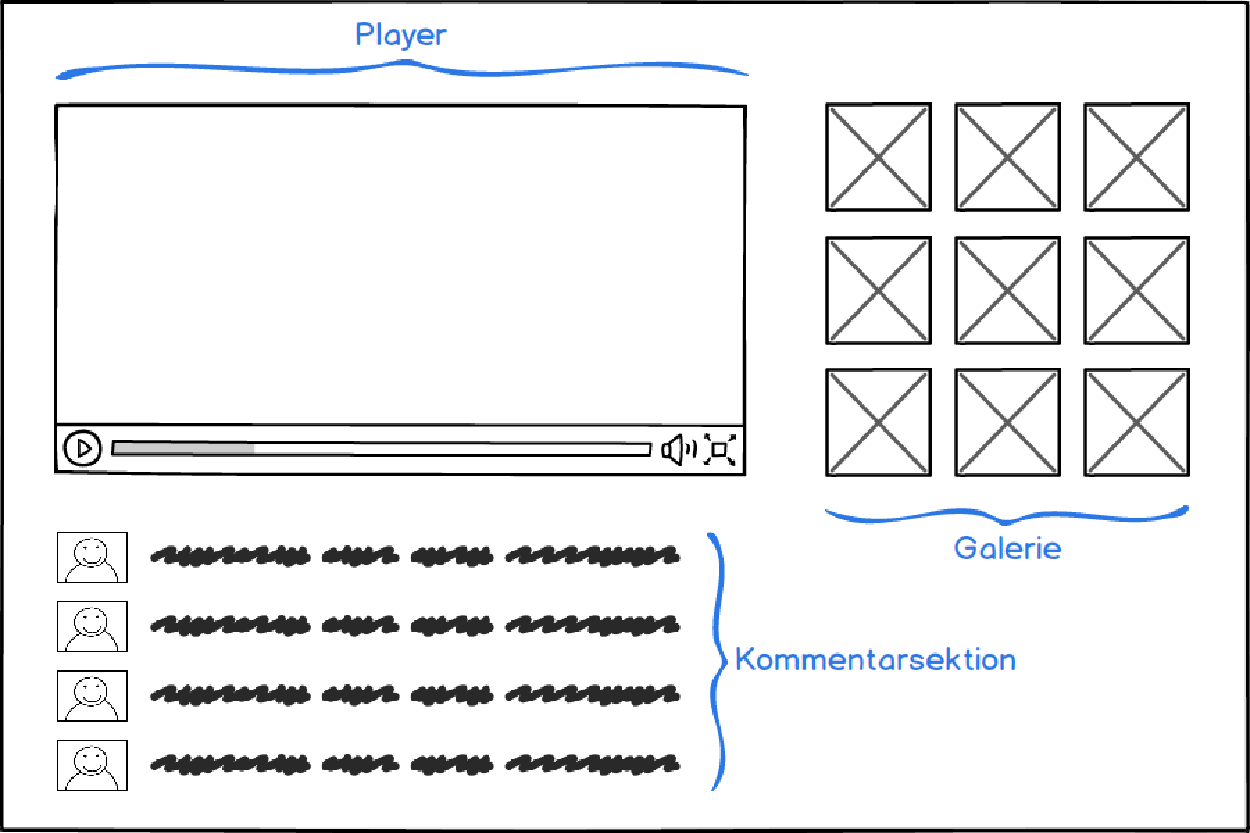
\includegraphics[width=.8\textwidth,center]{MockupBereiche.pdf}
\caption{\label{fig:MockupBereiche}Erste Skizze der Moodle-Repräsentation eines Hyperaudio-Dokuments}
\end{figure}

%Bevor nun die Bedürfnisse festgehalten werden, ist es zunächst sinnvoll das Plugin in mehrere Bereiche aufzuteilen. Hierbei scheint die Aufteilung in die Bereiche Schnittstelle, Integration in die Moodle-Oberfläche, Player für Hyperaudio-Dokumente und Kommentarfunktion plausibel.

%%%%%%%%%%
\section{Bedürfnisse der Studierenden und Lehrenden}
Bevor wir mit der detaillierten Konzeption des Plugins beginnen können, ist es wichtig, sich nochmals genauer mit den möglichen Bedürfnissen der Studierenden und Lehrenden auseinanderzusetzen. Eine Analyse der Bedürfnisse mittels Umfrage und/oder Interviews würde den Umfang dieser Arbeit sprengen, weshalb hierauf verzichtet wird.

Nun sollen im ersten Schritt die Anforderungen an die einzelnen Bereiche erarbeitet werden, wobei bereits die Gruppe der Betroffenen mit festgehalten werden soll. Nachdem die Anforderungen erfasst wurden, sollen diese im zweiten Schritt mit einer Priorität versehen werden. Diese wird dann herangezogen um bei der geplanten iterativen Programmierung die Reihenfolge, in der die Anforderungen umgesetzt werden, zu bestimmen.

%%%%%%%%%%
\subsection{Anforderungen an die Schnittstelle}
Die Schnittstelle soll es den Lehrenden ermöglichen, Hyperaudio-Dokumente in Moodle zu übertragen. Um die Anforderungen an die Schnittstelle zu ermitteln, überlegen wir kurz was ein Hyperaudio-Dokument ausmacht. Ein solches Dokument besteht zum einen aus einer Audio-Datei. Hieraus resultiert die Anforderung an die Schnittstelle, dass man festlegen können muss, welche Audio-Datei abgespielt werden soll. Zum anderen besteht ein Hyperaudio-Dokument aus zeitabhängigen Annotationen von Bildern, Tabellen, Formeln etc. Die Schnittstelle muss es uns also ermöglichen, zu definieren, zu welchem Zeitpunkt und für welche Dauer welches Zusatzinhalte angezeigt werden soll. Außerdem wäre es noch praktisch, Metadaten, wie den Autor, Quellen oder weiterführende Links, an das Hyperaudio-Dokument anzuheften. Um all diese Informationen zu speichern entsteht automatisch die Anforderung an eine Schnittstellen-Datei. Natürlich muss es auch die Möglichkeit geben, das Hyperaudio-Dokument in Moodle zu importieren. Alle diese Anforderungen (siehe Tabelle \ref{tab:AnforderungenSchnittstelle}) haben gemeinsam, dass ausschließlich die Lehrenden die Betroffenen darstellen.

\begin{table}[!ht]
\def\arraystretch{1.4}
\caption{Anforderungen an die Schnittstelle}
\label{tab:AnforderungenSchnittstelle}
 \begin{tabularx}{\textwidth}{lXl}      
    \hline
    Nr. & Anforderung & Betroffene 
    \\\hline
    1. & Definition einer Schnittstellen-Datei & \\
    1.1 & Definition der abzuspielenden Audiodatei & Lehrende\\
    1.2 & Definition der zeitabhängigen Annotationen (Bildern, Tabellen, Formeln etc.) & Lehrende\\
    1.3 & Definition von Metadaten (Autor, Quellen, weiterführende Links etc.) & Lehrende\\
    2. & Entwickeln eines Imports für Moodle & Lehrende\\
    \hline
    \end{tabularx}
\end{table}

%%%%%%%%%%
\subsection{Anforderungen an die Integration in die Moodle-Oberfläche}
\label{sub:AnforderungenOberflaeche}
Um die Anforderungen für die Integration in die Moodle-Oberfläche (siehe Tabelle \ref{tab:AnforderungenIntegration}) zu bestimmen, versuchen wir uns in die Studierenden und Lehrenden hineinzuversetzen. 

Zunächst beginnen wir mit der Perspektive der Lehrenden. Für diese Gruppe steht natürlich die Administration von Hyperaudio-Dokumenten im Vordergrund. Dementsprechend muss eine Administrationsseite zur Verfügung gestellt werden, über welche die Hyperaudio-Dokumente hochgeladen und verwaltet werden können.

Nun kommen wir zu den Anforderungen, die sowohl Lehrende als auch Studierende an die Integration stellen. Die zentrale Anlaufstelle, an denen die Lerninhalte für die Lehrenden und Studierenden angezeigt werden, ist natürlich die Kursseite des jeweiligen Kurses. Also muss die Darstellung der Hyperaudio-Dokumente in die Kursseiten integriert werden. Bei dieser Integration müssen wiederum neben der reinen Integration eines Players für Hyperaudio-Dokumente weitere Aspekte berücksichtigt werden. Eine weitere Anforderung könnte sein, dass alle dargestellten Zusatzinhalte in einer separaten Galerie dargestellt werden, damit sich schnell einen Überblick über diese gemacht werden kann und gegebenenfalls schnell wieder an die entsprechende Stelle im Hyperaudio-Dokument gesprungen werden kann. Hier ist also auch eine Rückkopplung zum Player notwendig. Des Weiteren muss hier auch die gewünschte Kommentarsektion eingebunden werden, über welche sich die Studierenden und Lehrenden untereinander austauschen können.

Zusätzlich ist auch eine Favoritenfunktion denkbar, mit welcher sich Studierende und Lehrende bestimmte Hyperaudio-Dokumente als Favoriten speichern können. Passend hierzu müsste es dann eine Übersicht über alle favorisierten Hyperaudio-Dokumente geben, welche ähnlich dargestellt werden könnte wie die bereits vorhandene Moodle-Ansicht \glqq Meine Lernumgebungen\grqq.

Eine Übersicht über alle zuletzt abgespielten Dokumente stellt eine ähnliche Anforderung dar.

Eine weitere mögliche Anforderung ist eine Übersichtsseite über alle verfügbaren Hyperaudio-Angebote aufgegliedert nach Kurs, Kurseinheit und Kapitel.

\begin{table}[!ht]
\def\arraystretch{1.4}
\caption{Anforderungen an die Integration in die Moodle-Oberfläche}
\label{tab:AnforderungenIntegration}
 \begin{tabularx}{\textwidth}{lXl}      
    \hline
    Nr. & Anforderung & Betroffene 
    \\\hline
    1. & Einbindung der Administration in die Kursseite & Lehrende\\
    2. & Einbindung der Hyperaudio-Dokumente in die Kursseite & \\
    2.1 & Einbindung des Players & Lehrende und Studierende\\
    2.2 & Einbindung einer Galerie der zeitabhängig annotierten Bilder, Tabellen, Formeln etc. mit Rückkopplung zum Player & Lehrende und Studierende\\
    2.3 & Einbindung der Kommentarsektion & Lehrende und Studierende\\
    3. & Favoritenfunktion analog zu \glqq Meine Lernumgebungen\grqq & Lehrende und Studierende\\
    4. & Übersicht über zuletzt abgespielte Hyperaudio-Dokumente & Lehrende und Studierende\\
    5. & Übersicht über alle verfügbaren Hyperaudio-Angebote & Lehrende und Studierende\\
    \hline
    \end{tabularx}
\end{table}

%%%%%%%%%%
\subsection{Anforderungen an die Kommentarsektion}
\label{sub:AnforderungenKommentarsektion}
Nachdem bereits bei den Anforderungen an die Intergration in die Moodle-Oberfläche auf die Kommentarsektion verwiesen wurde, sollen nun auch hierfür die Anforderungen definiert werden. Zunächst besteht der Wunsch, dass die Kommentarsektion neben öffentlichen Kommentaren auch persönliche Notizen enthalten können soll.

An dieser Stelle wollen wir die Unterscheidung zwischen öffentlichen Kommentaren, persönlichen Notizen und persönlichen Markierungen vornehmen. Öffentliche Kommentare stellen die übliche Art der Kommentare dar, mittels derer der Austausch unter den Studierenden und den Lehrenden stattfindet. Persönliche Notizen stellen eine spezielle Form der Kommentare dar. Diese sind im Grunde auf gleiche Art und Weise wie die öffentlichen Kommentare zu verstehen, mit der einzigen Ausnahme, dass diese nur durch den Verfasser eingesehen werden können. Persönliche Markierungen dagegen sollen dem Studierenden oder Lehrenden die Möglichkeit geben, bestimmte Zeitpunkte des Hyperaudio-Dokuments für eventuelle spätere Bearbeitungen vorzumerken. Markierungen werden nur innerhalb des Players vorgenommen, sodass diese keinen Bestandteil der Kommentarsektion darstellen. %Persönliche Markierungen dagegen sollen dem Studierenden und Lehrenden die Möglichkeit geben, eine im Player sichtbare Markierung innerhalb der Fortschrittsleiste vorzunehmen. Diese Markierungen stellen also keinen Bestandteil der Kommentarsektion dar.

%Am Anfang steht hier zunächst die Anforderung, dass Kommentare und persönliche Notizen erstellt werden können. Diese Kommentare und persönlichen Notizen sollen in der Kommentarsektion chronologisch dargestellt werden.
In der Kommentarsektion sollen Kommentare und Notizen chronologisch dargestellt werden.
% Dabei soll aus zwei Betrachtungsweisen entschieden werden können, zum einen der Betrachtung anhand des Erstellungsdatums und zum anderen mittels des Zeitpunktes zu dem der Kommentar oder die Notiz an das Hyperaudio-Dokument annotiert wurde.
Die Sortierung erfolgt standardmäßig anhand der Zeitpunkte, zu denen die Kommentare oder Notizen an das Hyperaudio-Dokument annotiert wurden. Alternativ kann der Betrachter auch eine Sortierung nach Erstellungsdatum wählen. 
Da die Studierenden und Lehrenden sich mittels der Kommentare austauschen können sollen, besteht auch die Anforderung, direkt auf einen öffentlichen Kommentar antworten zu können. Bei persönlichen Notizen besteht der Wunsch, diese auch bearbeiten und löschen zu können. Da jeder Kommentar und auch jede Notiz zu einem bestimmten Zeitpunkt innerhalb des Hyperaudio-Dokuments gehört, soll es auch möglich sein, vom jeweiligen Kommentar beziehungsweise von der jeweiligen Notiz aus zu der entsprechenden Stelle im Hyperaudio-Dokument zu springen. Diese Anforderung wird entsprechend in Tabelle \ref{tab:AnforderungenKommentarsektion} ergänzt. Zusätzlich wäre es auch von Vorteil, wenn in den Kommentare und Notizen nach Stichwörtern gesucht werden könnte.

\begin{table}[!ht]
\def\arraystretch{1.4}
\caption{Anforderungen an die Kommentarsektion}
\label{tab:AnforderungenKommentarsektion}
 \begin{tabularx}{\textwidth}{lXl}      
    \hline
    Nr. & Anforderung & Betroffene 
    \\\hline
    %1. & Erstellen von Kommentaren und persönlichen Notizen & Lehrende und Studierende\\
    1. & Chronologische Darstellung der Kommentare und Notizen & Lehrende und Studierende\\
    2. & Antworten auf öffentliche Kommentare & Lehrende und Studierende\\
    3. & Bearbeiten persönlicher Notizen & Lehrende und Studierende\\
    4. & Löschen persönlicher Notizen & Lehrende und Studierende\\
    5. & Rückkopplung zum Player & Lehrende und Studierende\\
    6. & Suchfunktion in den Kommentaren und Notizen & Lehrende und Studierende\\
    \hline
    \end{tabularx}
\end{table}

%%%%%%%%%%
\subsection{Anforderungen an den Player für Hyperaudio-Dokumente}
Wenden wir uns nun den Anforderungen an den Player zu. Hierbei macht es wieder Sinn sich zu überlegen was mit dem Hyperaudio-Dokument bezweckt werden soll. Die Grundfunktion des Players besteht darin, Audio-Dateien abzuspielen. Zusätzlich sollen die zeitabhängig annotierten Zusatzinhalte dargestellt werden. Zu dem Zeitpunkt, zu dem die Zusatzinhalte dargestellt werden, ist die Wiedergabe eines \textit{Audio Cues}, also eines akustischen Hinweises, gewünscht, der die Zuhörer auf die Anzeige der annotierten Zusatzinhalte aufmerksam macht. Eine weitere Anforderung ist die Einbettung der Kommentare und Notizen in den Player. Diese besteht zum einen aus der reinen Visualisierung der zeitabhängig annotierten Kommentare und Notizen, zum anderen werden auch Interaktionsmöglichkeiten geboten, sei es die Weiterleitung an die entsprechende Stelle in der Kommentarsektion oder die Erstellung neuer zeitabhängiger annotierter Kommentare und Notizen.  Auch das Erstellen und Löschen von persönlichen Markierungen innerhalb des Players samt derer Visualisierung stellt eine Anforderung an den Player dar und wird in Tabelle \ref{tab:AnforderungenPlayer} festgehalten.

Vorstellbar ist darüber hinaus, dass der Player sich beim Schließen der Seite merkt, zu welchem Zeitpunkt das Hyperaudio-Dokument beendet wurde, um es beim erneuten Öffnen an ebendieser Stelle fortzusetzen.

\begin{table}[!ht]
\def\arraystretch{1.4}
\caption{Anforderungen an den Player für Hyperaudio-Dokumente}
\label{tab:AnforderungenPlayer}
 \begin{tabularx}{\textwidth}{lXl}      
    \hline
    Nr. & Anforderung & Betroffene 
    \\\hline
    1. & Wiedergabe der Audiodatei & Lehrende und Studierende\\
    2. & Darstellung der zeitabhängig annotierten Bilder, Tabellen, Formeln etc & Lehrende und Studierende\\
    3. & Wiedergabe der Audio Cues & Lehrende und Studierende\\
    4. & Einbettung der Kommentare und Notizen & \\
    4.1 & Visualisierung der zeitabhängig annotierten Kommentare und Notizen & Lehrende und Studierende\\
    4.2. & Interaktionsmöglichkeiten & \\
    4.2.1 & Weiterleitung zu vorhandenen Kommentaren und Notizen in der Kommentarsektion  & Lehrende und Studierende\\
    4.2.2 & Erstellen zeitabhängiger annotierter Kommentare und Notizen & Lehrende und Studierende\\
    5. & Einbettung der persönlichen Markierungen & \\
    5.1 & Visualisierung der zeitabhängig annotierten Markierungen & Lehrende und Studierende\\
    5.2. & Interaktionsmöglichkeiten & \\
    5.2.1 & Erstellen zeitabhängig annotierter Markierungen  & Lehrende und Studierende\\
    5.2.2 & Löschen zeitabhängig annotierter Markierungen & Lehrende und Studierende\\
    6. & Funktion zum Fortsetzen unterbrochener Wiedergaben bei folgenden Aufrufen in Moodle & Lehrende und Studierende\\
    \hline
    \end{tabularx}
\end{table}

%%%%%%%%%%
\subsection{Priorisierung der Anforderungen}
Im nächsten Schritt nehmen wir die Priorisierung der erfassten Anforderungen vor. Hierbei wird bewertet wie wichtig der in der Anforderung beschriebene Wunsch für die Erreichung des Lernziels ist. Die Priorisierung wird anhand der drei Prioritätsstufen \textit{niedrig}, \textit{mittel} und \textit{hoch} festgelegt.

\subsubsection{Priorisierung: Anforderungen an die Schnittstelle}
Wenn die gesammelten Anforderungen an die Schnittstelle betrachtet werden, kann festgestellt werden, dass abgesehen von der Definition von Metadaten (Autor, Quellen, weiterführende Links etc.) alle Anforderungen essenziell für die Erreichung des Lernziels und somit zur Umsetzung des Plugins sind. Die Metadaten stellen aber dennoch sinnvolle Informationen bereit, welche dem Studierenden beim Erreichen des Lernziels helfen können. Daraus resultiert die in Tabelle \ref{tab:PriorisierungAnforderungenSchnittstelle} dargestellte Priorisierung.

\begin{table}[!ht]
\def\arraystretch{1.4}
\caption{Priorisierung: Anforderungen an die Schnittstelle}
\label{tab:PriorisierungAnforderungenSchnittstelle}
 \begin{tabularx}{\textwidth}{lXll}      
    \hline
    Nr. & Anforderung & Betroffene & Priorität
    \\\hline
    1. & Definition einer Schnittstellen-Datei & & \\
    1.1 & Definition der abzuspielenden Audiodatei & Lehrende & hoch\\
    1.2 & Definition der zeitabhängigen Annotationen (Bildern, Tabellen, Formeln etc.) & Lehrende & hoch\\
    1.3 & Definition von Metadaten (Autor, Quellen, weiterführende Links etc.) & Lehrende & mittel\\
    2. & Entwickeln eines Imports für Moodle & Lehrende & hoch\\
    \hline
    \end{tabularx}
\end{table}

%%%%%%%%%%
\subsubsection{Priorisierung: Anforderungen an die Integration in die Moodle-Oberfläche}
Bei der Integration in die Moodle-Oberfläche ergibt sich eine Priorisierung in drei Stufen. Auf die Einbindung der Administration in die Kursseite kann nicht verzichtet werden, genauso wie auf die Einbindung der Hyperaudio-Dokumente in die Kursseite inklusive des Players und der Kommentarsektion. Demzufolge erhalten diese Anforderungen die Priorität \textit{hoch}. Der Anforderung \glqq Einbindung einer Galerie der zeitabhängig annotierten Bilder, Tabellen, Formeln etc. mit Rückkopplung zum Player\grqq{} wird die Priorität \textit{mittel} zugeordnet, da sie das Erreichen des Lernziels sehr wohl unterstützen kann, aber nicht zwangsweise dafür benötigt wird. Alle weiteren Anforderungen an die Integration in die Moodle-Oberfläche werden mit der Priorität \textit{niedirg} in Tabelle \ref{tab:PriorisierungAnforderungenIntegration} festgehalten, da sie nicht dem eigentlichen Erreichen des Lernziels dienen, sondern nur eine verbesserte Übersicht über die Hyperaudio-Dokumente bieten.

\begin{table}[!ht]
\def\arraystretch{1.4}
\caption{Priorisierung: Anforderungen an die Integration in die Moodle-Oberfläche}
\label{tab:PriorisierungAnforderungenIntegration}
 \begin{tabularx}{\textwidth}{lXll}      
    \hline
    Nr. & Anforderung & Betroffene & Priorität
    \\\hline
    1. & Einbindung der Administration in die Kursseite & Lehrende & hoch\\
    2. & Einbindung der Hyperaudio-Dokumente in die Kursseite & \\
    2.1 & Einbindung des Players & Lehrende und Studierende & hoch\\
    2.2 & Einbindung einer Galerie der zeitabhängig annotierten Bilder, Tabellen, Formeln etc. mit Rückkopplung zum Player & Lehrende und Studierende & mittel\\
    2.3 & Einbindung der Kommentarsektion & Lehrende und Studierende & hoch\\
    3. & Favoritenfunktion analog zu \glqq Meine Lernumgebungen\grqq & Lehrende und Studierende & niedrig\\
    4. & Übersicht über zuletzt abgespielte Hyperaudio-Dokumente & Lehrende und Studierende & niedrig\\
    5. & Übersicht über alle verfügbaren Hyperaudio-Angebote & Lehrende und Studierende & niedrig\\
    \hline
    \end{tabularx}
\end{table}

%%%%%%%%%%
\subsubsection{Priorisierung: Anforderungen an die Kommentarsektion}
Der Hauptbestandteil der Kommentarsektion besteht aus der Darstellung der Kommentare und Notizen. Die Vergabe einer hohen Priorität für diese Anforderung (siehe Tabelle \ref{tab:PriorisierungAnforderungenKommentarsektion}) ist daher trivial. Die Möglichkeit direkt auf Kommentare zu antworten und die Möglichkeit persönliche Notizen zu löschen stellen sinnvolle Erweiterungen der Kommentarfunktion dar, welche das Erreichen des Lernziels erleichtern können. Dies rechtfertigt die Priorität \textit{mittel}. Dem Bearbeiten persönlicher Notizen wird die Priorität \textit{niedrig} zugewiesen, da dieselben Ergebnisse auch dadurch erzielt werden können, dass ein bestehender Kommentar gelöscht und ein neuer Kommentar erstellt wird. Eine Bearbeitungsfunktion eröffnet also keine neuen Möglichkeiten, stellt jedoch eine Erleichterung des Arbeitsschrittes dar. Der Anforderung \glqq Rückkopplung zum Player\grqq{} wird die Priorität \textit{mittel} zugeordnet, da sie, ähnlich wie die Galerie, das Erreichen des Lernziels unterstützen kann, aber nicht zwangsweise dafür benötigt wird.
%Da der Fokus bei den Kommentaren von Hyperaudio-Dokumenten auf der Zeit und nicht direkt auf dem Inhalt liegt wird der Suchfunktion nur eine geringe Priorität zugewiesen
Eine Suchfunktion innerhalb der Kommentare ist nützlich, um Inhalte zu bestimmten Themen zu finden. Die Kommentare können jedoch auch anhand der Visualisierung im Player oder über die Inhalte der Galerie angesteuert werden. Da die Suchfunktion demnach nicht die einzige Möglichkeit darstellt, um zu den gewünschten Kommentaren zu navigieren, wird dieser nur eine geringe Priorität zugewiesen.

\begin{table}[!ht]
\def\arraystretch{1.4}
\caption{Priorisierung: Anforderungen an die Kommentarsektion}
\label{tab:PriorisierungAnforderungenKommentarsektion}
 \begin{tabularx}{\textwidth}{lXll}      
    \hline
    Nr. & Anforderung & Betroffene & Priorität
    \\\hline
    %1. & Erstellen von Kommentaren und persönlichen Notizen & Lehrende und Studierende & hoch\\
    1. & Chronologische Darstellung der Kommentare und Notizen & Lehrende und Studierende & hoch\\
    2. & Antworten auf öffentliche Kommentare & Lehrende und Studierende & mittel\\
    3. & Bearbeiten persönlicher Notizen & Lehrende und Studierende & niedrig\\
    4. & Löschen persönlicher Notizen & Lehrende und Studierende & mittel\\
    5. & Rückkopplung zum Player & Lehrende und Studierende & hoch\\
    6. & Suchfunktion in den Kommentaren und Notizen & Lehrende und Studierende & niedrig\\
    \end{tabularx}
\end{table}

%%%%%%%%%%
\subsubsection{Priorisierung: Anforderungen an den Player für Hyperaudio-Dokumente}
Beim Player stellen die Wiedergabe der Audiodatei und die Darstellung der zeitabhängig annotierten Bilder, Tabellen, Formeln etc. die essenziellen Funktionen dar und werden entsprechend mit der Priorität \textit{hoch} bewertet. Mit dem Hintergrund, dass die Studierenden während des Abspielens des Hyperaudio-Dokuments andere Tätigkeiten ausüben können und nur in bestimmen Momenten auf den PC blicken müssen sollen, kann auch die Anforderung \glqq Wiedergabe der Audio Cues\grqq{} mit der Priorität \textit{hoch} bedacht werden. Es ist zu betonen, dass die Kommentarfunktion einen wesentlichen Bestandteil des Plugins ausmachen soll. Um die Nutzung der Kommentarfunktion beim Abspielen der Dokumente möglichst komfortabel zu gestalten, sollten die Interaktionsmöglichkeiten entsprechend mit der Priorität \textit{hoch} versehen werden. Gleiches gilt für die Anforderungen bezüglich der persönlichen Markierungen. Die Visualisierung der Kommentare, Notizen und Markierungen an sich wird ebenfalls mit der Priorität \textit{hoch} bewertet.
% Das Erreichen des Lernzieles wird dadurch erleichtert, dass beim Abspielen des Dokuments schnell die gewünschten Aktionen ausgeführt werden können und somit weniger kostbare Lernzeit verschwendet wird.
Durch die Umsetzung der eben genannten Anforderungen können beim Abspielen des Dokuments schnell die gewünschten Aktionen ausgeführt werden, wodurch letztlich das Erreichen des Lernzieles erleichert wird.
Der Funktion zum Fortsetzen unterbrochener Wiedergaben bei folgenden Aufrufen in Moodle wird eine geringere Bedeutung zugeschrieben, da falls gewünscht beispielsweise auch mittels einer persönlichen Notiz oder Markierung der Zeitpunkt festgehalten werden kann, an dem das Dokument beim nächsten Aufruf fortgesetzt werden soll. Dementsprechend wird dieser Anforderung in Tabelle \ref{tab:PriorisierungAnforderungenPlayer} nur eine geringe Priorität zugeordnet.

\begin{table}[!ht]
\def\arraystretch{1.4}
\caption{Priorisierung: Anforderungen an den Player für Hyperaudio-Dokumente}
\label{tab:PriorisierungAnforderungenPlayer}
 \begin{tabularx}{\textwidth}{lXll}      
    \hline
    Nr. & Anforderung & Betroffene & Priorität
    \\\hline
    1. & Wiedergabe der Audiodatei & Lehrende und Studierende & hoch\\
    2. & Darstellung der zeitabhängig annotierten Bilder, Tabellen, Formeln etc. & Lehrende und Studierende & hoch\\
    3. & Wiedergabe der Audio Cues & Lehrende und Studierende & hoch\\
    4. & Einbettung der Kommentare und Notizen & \\
    4.1 & Visualisierung der zeitabhängig annotierten Kommentare und Notizen & Lehrende und Studierende & hoch\\
    4.2. & Interaktionsmöglichkeiten & \\
    4.2.1 & Weiterleitung zu vorhandenen Kommentaren und Notizen in der Kommentarsektion  & Lehrende und Studierende & hoch\\
    4.2.2 & Erstellen zeitabhängiger annotierter Kommentare und Notizen & Lehrende und Studierende & hoch\\
    5. & Einbettung der persönlichen Markierungen & \\
    5.1 & Visualisierung der zeitabhängig annotierten Markierungen & Lehrende und Studierende & hoch\\\\
    5.2. & Interaktionsmöglichkeiten & \\
    5.2.1 & Erstellen zeitabhängig annotierter Markierungen  & Lehrende und Studierende & hoch\\
    5.2.2 & Löschen zeitabhängig annotierter Markierungen & Lehrende und Studierende & hoch\\
    6. & Funktion zum Fortsetzen unterbrochener Wiedergaben bei folgenden Aufrufen in Moodle & Lehrende und Studierende & niedrig\\
    \hline
    \end{tabularx}
\end{table}

%%%%%%%%%%
\section{Lernen mit Hypermedia}
Bevor wir uns der genauen Konzeption und Implementation des Moodle Plugins für Hyperaudio-Dokumente zuwenden, betrachten wir zunächst \textit{Hypermedia} im Allgemeinen. Dabei wollen wir zunächst eine Begriffsklärung durchführen. Darauf aufbauend werden einige Erfahrungen aus verschiedenen wissenschaftlichen Arbeiten gesammelt. Zuletzt wollen wir hieraus einige Rückschlüsse für unser Moodle Plugin und unsere Interpretation von Hyperaudio ziehen.

%%%%%%%%%%
\subsection{Begriffsklärung}
Hyperaudio stellt eine Ausprägung von \textit{Hypermedia} dar. Der Begriff \textit{Hypermedia} wurde das erste Mal von Ted Nelson 1965 verwendet \citep{nelson1965complex}. In seinem Paper beschreibt er detailliert, was er sich unter einem \textit{Hypertext} vorstellt. Hierunter versteht er ein Dokument bestehend aus geschriebenen oder bildhaften Inhalten, welche in solch einer komplexen Art und Weise miteinander verbunden sind, dass sie nicht mehr auf Papier dargestellt werden können. Es kann Zusammenfassungen, Karten über die Inhalte und deren Zusammenhänge, Annotationen, Ergänzungen oder Anmerkungen von Wissenschaftlern, die das Dokument begutachtet haben, enthalten. Nelson beschreibt das Kriterium für den Präfix \textit{hyper} damit, dass diese Objekte nicht durch eine Konvertierung in ein einfaches lineares Medium, wie beispielsweise einen String umgewandelt werden können. Der wesentliche Punkt ist also, dass es sich beim Lernen mit \textit{Hypermedia} um ein nicht-lineares Lernen handelt.

Genauer betrachtet stellt das, was Nelson sich damals als \textit{Hypertext} vorgestellt hatte, nach heutiger Definition bereits eine Form von \textit{Hypermedia} dar. Auch wenn viele die beiden Begriffe \textit{Hypertext} und \textit{Hypermedia} synonym verwenden \citep{nielsen2013multimedia}, werden bei strikter Betrachtung bei \textit{Hypertext} ausschließlich Texte miteinander verbunden, während bei \textit{Hypermedia} auch andere Medien eingebunden werden können. Gemeinsam haben beide Arten jedoch, dass der Lernende keinen linearen Weg vorgegeben hat, sondern von einem Knoten (Node) zum anderen springen kann und sich somit seinen Lernweg selbst aussucht. Als Folge dessen stellt \textit{Hypermedia} eine nicht-lineare Variante von \textit{Multimedia} dar.

Nach dieser Logik handelt es sich bei Hyperaudio in seiner klassischen Form eigentlich um reine Audiosequenzen, die miteinander verknüpft sind, wobei der Lernende selbst entschieden kann, in welcher Reihenfolge er diese abspielt \citep{zumbach2006learning}.

%%%%%%%%%%
\subsection{Erfahrungen}
Die Wissenschaft beschäftigt sich schon seit vielen Jahren damit, festzustellen, welche Effekte der Einsatz von \textit{Multimedia}, \textit{Hypertext} und \textit{Hypermedia} auf den Lernerfolg von Lehrenden hat. In der Arbeit von \cite{moos2010multimedia} wird eine Analyse von etlichen Arbeiten zu diesem Thema durchgeführt. \cite{moos2010multimedia} konzentrieren sich hierbei vor allem auf den Einfluss auf die Motivation der Lernenden. Dennoch wird auch auf andere Aspekte der drei verschiedenen E-Learning Methoden \textit{Multimedia}, \textit{Hypertext} und  \textit{Hypermedia} im Vergleich zu klassischen Lehrmethoden eingegangen.

\cite{moos2010multimedia} verweisen auf Arbeiten, nach denen eine Herausforderung bei \textit{Multimedia} und somit auch bei \textit{Hypermedia} darin besteht, dass die kognitive Aufnahmekapazität der Studierenden überschritten werden kann (Mayer und Moreno; van Merrienboer und Ayres, nach \cite{moos2010multimedia}), wenn Informationen sowohl aus einem Text als auch aus einem Diagramm entnommen werden sollen. Dies beruht auf der Annahme der Cognitive Load Theory, welche dem Arbeitsgedächtnis nur eine begrenzte Kapazität zuspricht (Sweller; van Merrienboer und Sweller, nach \cite{moos2010multimedia}). Es gibt aber auch Studien, welche einen positiven Effekt nachweisen, wenn zur gleichen Zeit Bilder dargestellt werden und dazu passender Text vorgelesen wird, im Vergeleich zum alleinigen Betracheten von Bildern beziehungsweise Anhören von Texten (Mayer und Anderson; Mayer und Sims, nach \cite{moos2010multimedia}).

\textit{Hypertext} bietet zwar Vorteile, da der Studierende den Lernweg bestimmen kann, der am besten auf seine Bedürfnisse angepasst ist. Auf der anderen Seite ist hierzu aber eine ausreichende Vorkenntnis in dem Lernbereich notwendig, um die Entscheidung, wie dieser Weg aussehen soll treffen zu können. Des Weiteren wirkt sich auch ein fehlendes Interesse des Studierenden negativ auf die Effektivität der \textit{Hypertext} Lernumgebung aus (Lawless und Kulikowich, nach \cite{moos2010multimedia}).
\todo[inline]{Zitat nochmals prüfen}

Es ist nun also nicht verwunderlich, dass \textit{Hypermedia} als Verschmelzung von \textit{Multimedia} und \textit{Hypertext} ebenfalls einige Herausforderungen mit sich bringt \citep{moos2010multimedia}. Scott und Schwartz (nach \cite{moos2010multimedia}) fordern für das Lernen mit \textit{Hypermedia} eine Balance zwischen effektiver Navigation und Inhaltsverständnis. Dies soll durch Prozesse zur Überwachung des eigenen Lernfortschritts erreicht werden, doch Untersuchungen haben ergeben, dass viele Studierende Schwierigkeiten haben diese Prozesse korrekt anzuwenden \citep{moos2010multimedia}.


%%%%%%%%%%
\subsection{Rückschlüsse}
Nachdem wir nun die Begrifflichkeiten um \textit{Hypermedia}, sowie den Begriff Hyperaudio im eigentlichen Sinne beleuchtet und entsprechende Studien betrachtet haben, gehen wir nun darauf ein, welche Rückschlüsse daraus für diese Arbeit gezogen werden können.

Zum einen stellen wir fest, dass wir den Begriff Hyperaudio nicht im ursprünglichen Sinn verwenden. Bei unseren Hyperaudio-Dokumenten handelt es sich eigentlich um Multimedia-Dokumente. Erst unter Berücksichtigung der Kommentarfunktion und der Galerie wird der Hypermedia-Aspekt erfüllt. Der Zuhörer hat also die Möglichkeit von Kommentar zu Kommentar oder von Annotation zu Annotation zu springen und gelangt dabei an die entsprechende Stelle in der Audiosequenz. Im Gegensatz zu \cite{zumbach2006learning} verstehen wir unter Hyperaudio eine Audio-Datei, die durch die Erweiterung mittels Annotationen und Kommentarfunktion um Multimedia- und Hypermedia-Elemente ergänzt wird.

Der Vorteil unserer Betrachtungsweise von Hyperaudio liegt darin, dass die Herausforderungen, die in Verbindung mit \textit{Hypermedia} bzw. \textit{Hypertext} normalerweise auftreten, nicht besonders prägnant sind. In unserem Plugin wird dem Studierenden in erster Linie eine lineare Audio-Datei vorgespielt, die um Multimedia-Elemente ergänzt wird. Erst durch den Einsatz der Galerie und der Kommentarfunktion kommen die herausfordernden Elemente von Hypermedia ins Spiel. Dementsprechend sollte unser Hyperaudio-Plugin einen guten Kompromiss zwischen den verschiedenen Lehrmethoden darstellen.

%%%%%%%%%%
\section{Zusammenhänge der medialen Komponenten von Hyperaudio-Dokument und Annotationen}
In diesem Abschnitt wollen wir nochmals genauer auf den Aufbau eines Hyperaudio-Dokuments im Sinne dieser Arbeit eingehen. Hierbei soll vor allem geklärt werden, wie die einzelnen Komponenten zusammenhängen und welche Möglichkeiten dadurch gegeben beziehungsweise nicht gegeben sind.

%%%%%%%%%%
\subsection{Komponenten}
Im Mittelpunkt eines Hyperaudio-Dokument steht eine Audio-Datei. Inhaltlich kann es sich hierbei beispielsweise um einen Vorlesungsvortrag handeln. Man könnte sich auch vorstellen, dass ein Hyperaudio-Dokument aus mehreren aneinandergereihten Audio-Dateien besteht. Dies würde an der grundsätzlichen Problemstellung jedoch nichts ändern und kann im Nachhinein jederzeit als Erweiterung umgesetzt werden. Aus diesem Grund wird in dieser Arbeit nur ein Plugin für ein Hyperaudio-Dokument bestehend aus einer Audio-Datei entwickelt.

Neben dieser zentralen Audio-Datei besteht das Hyperaudio-Dokument aus mehreren Zusatzinhalten, wobei es sich um Bilder, Graphen, Tabellen usw. handeln kann. Entscheidend ist aber, dass diese Zusatzinhalte immer nur eine rein grafische Darstellung verkörpern. Videos mit Ton sind somit beispielsweise nicht als Zusatzinhalt verwendbar, reine Animationen ohne Ton sind aber durchaus möglich.

Als besondere, nämlich externe Komponente, sind die Kommentare zu nennen. Diese gehören nicht zum eigentlichen Hyperaudio-Dokument, sollen aber mit diesem verknüpft werden. Es wird drei verschiedene Arten von Kommentaren geben, nämlich  öffentliche Kommentare, persönliche Notizen und persönliche Markierungen.  Innerhalb der öffentlichen Kommentare muss noch zwischen den Original-Kommentaren und den Antworten auf diese unterschieden werden. 


%%%%%%%%%%
\subsection{Zusammenhänge}
Zunächst betrachten wir den Zusammenhang zwischen Audio-Datei und den Zusatzinhalten. Zu jedem beliebigen Zeitpunkt innerhalb der Abspieldauer der Audio-Datei kann maximal ein Zusatzinhalt gleichzeitig annotiert werden. Es sind also auch Phasen möglich zu denen keinerlei Zusatzinhalt dargestellt wird. Das Zeitfenster für die Annotation soll mittels einer Start- und Endzeit pro Zusatzinhalt definiert werden, wobei nur die Minuten und Sekunden anzugeben sind. Bei dem Zeitfenster sollte natürlich bedacht werden, dass dieses nicht zu kurz sein sollte. Zwar soll, sobald ein Zusatzinhalt im Player des Hyperaudio-Dokuments angezeigt wird,  ein entsprechender Audio Cue abgespielt werden, dennoch können bereits einige Sekunden vergehen bis der Studierende seinen Blick dem Player zuwendet.

Auch die Kommentare stehen als externe Komponente in einer gewissen Art und Weise im Zusammenhang mit der Audio-Datei. Dies ergibt sich daraus, dass Kommentare zu einem bestimmten Zeitpunkt innerhalb der Audio-Datei erfasst werden. Während Antworten auf Original-Kommentare erfasst werden können, sind Antworten auf Antworten nicht möglich.

Zwischen Kommentaren und Zusatzinhalten gibt es jedoch keinen direkten Zusammenhang. Solche Zusammenhänge ergeben sich alleine aus den Zeitpunkten der Annotationen. Zusatzinhalte können wiederum in keinem Zusammenhang mit einem anderen Zusatzinhalt stehen.

Diese Zusammenhänge sind im UML-Diagramm in Abbildung \ref{fig:UMLAufbau} ersichtlich.

\begin{figure}[h!]
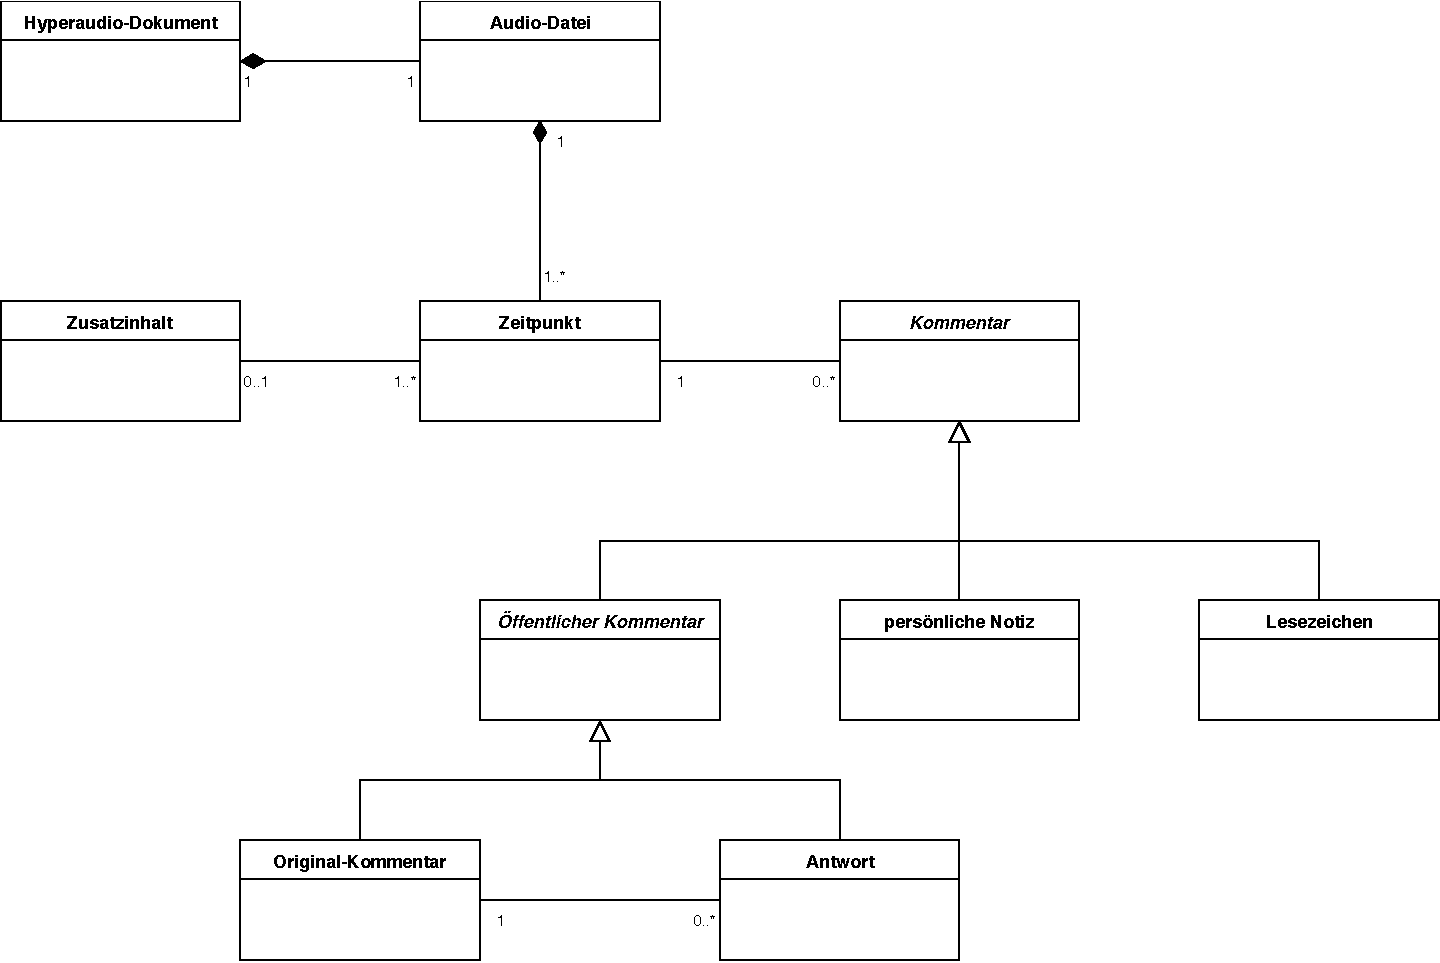
\includegraphics[width=\textwidth,center]{UMLZusammenhaenge.pdf}
\caption{\label{fig:UMLAufbau}Zusammenhänge der Komponenten}
\end{figure}


%%%%%%%%%%
\section{Evaluation bestehender Komponenten}
Bevor wir mit der Konzeption und Implementierung unseres Moodle-Plugins beginnen, wenden wir uns nun der Evaluation bestehender Komponenten zu. Ziel ist es festzustellen, ob eventuell bereits Technologien existieren, mit deren Hilfe unsere Idee des Moodle-Plugins umgesetzt werden kann oder ob zumindest Teile davon - unter entsprechender Beachtung der Lizenzierung - sinnvoll wiederverwendet werden können. Wir gehen hierbei so vor, dass wir die einzelnen vorhanden Technologien auf diesem Gebiet und ihre Funktionen vorstellen und anschließend bewerten, inwiefern diese für die Umsetzung des Plugins relevant sind.

%%%%%%%%%%
\subsection{VideoJS Player}
Bei dem \textit{VideoJS Player}\footnote{GitHub-Projekt, Apache-Lizenz 2.0: http://videojs.com/; https://github.com/videojs} handelt es sich um eine Open Source Bibliothek zum Abspielen von Videos und stellt damit einen HTML5 Video Player zur Verfügung. Der \textit{VideoJS Player} ist bereits als Standard Plugin für die Wiedergabe von Audio- und Video-Dateien in Moodle integriert. Wie der Name schon erkennen lässt, handelt es sich hierbei um eine JavaSrcipt Bibliothek. Der \textit{VideoJS Player} beschränkt sich in seiner Ausgangsversion ausschließlich auf das Abspielen von Audio- und Video-Dateien und bietet bis auf ein optionales Fallback auf den Adobe FlashPlayer keine weiteren Funktionen. Die Funktionalität des \textit{VideoJS Player} kann aber über Plugins erweitert werden. Es existieren bereits zahlreiche solcher Plugins. Hier sei vor allem das Plugin \textit{videojs-wavesurfer}\footnote{GitHub-Projekt, MIT Lizenz: https://github.com/collab-project/videojs-wavesurfer} zu nennen, welches das wavesurfer.js Framework (siehe Abschnitt \ref{sec:wavesurfer.js}) in den \textit{VideoJS Player} einbindet. Dank der Unterstützung von Plugins ist es durchaus denkbar, den Player mittels Plugin beispielsweise um Buttons zum Erstellen von Kommentaren oder persönlichen Notizen zu erweitern. Auch wäre es denkbar, mittels eines Plugins die annotierten Kommentare zu visualisieren. Grundsätzlich stellt der \textit{VideoJS Player} somit eine gute Ausgangslage für einen Hyperaudio-Player dar.

%%%%%%%%%%
\subsection{H5P}
Mit \textit{H5P} und dem bereits vorhanden Plugin für Moodle\footnote{GitHub-Projekt, GNU General Public License v2.0: https://github.com/h5p/h5p-moodle-plugin} ist es möglich, etliche verschieden Arten von interaktiven Lerninhalten zu gestalten. Dabei handelt es sich um eine Sammlung von interaktiven Komponenten, darunter Course Presentation, Timeline und Interactive Video. Course Presentation bietet die Möglichkeit, interaktive Präsentationen zu gestalten. Timeline kann genutzt werden um Inhalte anhand eines Zeitstrahls darzustellen. Interactive Video ermöglicht, ähnlich wie Course Presentation, die Interaktion während des Abspielens eines Videos. Besonders erwähnenswert ist, dass sich bei \textit{H5P} die interaktiven Inhalte innerhalb der Weboberfläche erstellen lassen. Es wäre also denkbar, eine eigene interaktive Komponente zu entwickeln, welche es ermöglicht, Hyperaudio-Dokumente als interaktiven Lerninhalt zu erstellen und abzuspielen.

%%%%%%%%%%
\subsection{Popcorn.js}
Die Mozilla Corporation bietet mit \textit{Popcorn.js}\footnote{GitHub-Projekt, MIT Lizenz: https://github.com/mozilla/popcorn-js} eine Bibliothek an, welche neben einer standardisierten Steuerung von Medieninhalten aus verschiedenen Quellen auch die Annotation von Inhalten mittels Plugins ermöglicht. Hier wäre also auch eine Entwicklung eines Plugins denkbar, mit welchem wir unsere Hyperaudio-Dokumente wie gewünscht wiedergeben könnten. Die Wartung für die Bibliothek wurde seitens Mozilla zwar eingestellt, das Projekt steht aber weiterhin auf GitHub zur Verfügung. Obwohl das Projekt nicht mehr weiterentwickelt wird, kann es durch die vorhandenen Steuerungsmöglichkeiten und das Plugin-System ein sehr geeignetes Grundgerüst für die Entwicklung unseres Moodle Plugins darstellen.
 
%%%%%%%%%%
\subsection{wavesurfer.js}
\label{sec:wavesurfer.js}
Bei \textit{wavesurfer.js}\footnote{GitHub-Projekt, BSD-3-Clause: https://wavesurfer-js.org; https://github.com/katspaugh/wavesurfer.js} handelt es sich um ein JavaScript Framework, welches es ermöglicht, die Wellenform zu der abgespielten Audio-Datei in einem Audio-Player visualisieren zu lassen. Diese Basisfunktionalität wurde durch Weiterentwicklungen um nützliche Funktionen erweitert. Auf zwei dieser Weiterentwicklungen gehen wir im Folgenden ein.

%%%%%%%%%%
\subsubsection{audio-annotator}
Der \textit{audio-annotator} stellt eine auf dem \textit{wavesurfer.js} Framework basierende Weiterentwicklung dar, welche es mittels Weboberfläche ermöglicht, Annotationen in Form von Text an eine Audio-Datei anzuheften. Es erweitert \textit{wavesurfer.js} also um die Möglichkeit, Annotationen an eine Datei anzuheften und bietet gleichzeitig noch eine Oberfläche, um ebendiese Annotationen vorzunehmen.

%%%%%%%%%%
\subsubsection{BAT - BMAT Annotation Tool}
Beim \textit{BAT - BMAT Annotation Tool}\footnote{GitHub-Projekt, GNU General Public License 3: https://wavesurfer-js.org; https://github.com/BlaiMelendezCatalan/BAT} handelt es sich um eine Entwicklung basierend auf der im Zusammenhang von \textit{audio-annotator} erweiterten Frameworks \textit{wavesurfer.js} und \textit{regions.js}. Es ermöglicht, ebenso wie \textit{audio-annotator}, dem Benutzer mittels Weboberfläche Annotationen an einer Audio-Datei vorzunehmen. Somit bietet \textit{BAT - BMAT Annotation Tool} logischerweise dieselben Vorzüge wie bereits der \textit{audio-annotator}. Im Vergleich zum \textit{audio-annotator} stellt \textit{BAT - BMAT Annotation Tool} jedoch ein weiterentwickelteres Framework dar.

\todo[inline]{regions.js bereits bei audio-annotator in Verwendung?}

\subsubsection{wavesurfer.js für Hyperaudio-Dokumente}
Das \textit{wavesurfer.js} Framework - speziell mit seinen Weiterenticklungen - bietet einige Funktionen, die für das Abspielen von Hyperaudio-Dokumenten nützlich sein könnten. Zusätzlich bietet es auch die Funktion,  die entsprechenden Annotationen in einer Weboberfläche an die Audio-Dateien anzuheften. Grundsätzlich lässt sich feststellen, dass \textit{wavesurfer.js} und seine Ableger im Vergleich zu den zuvor betrachteten Entwicklungen einen wesentlich unausgereifteren Eindruck hinterlassen.

%%%%%%%%%%
\subsection{timesheets.js}
\textit{timesheets.js}\footnote{ehemaliges GitHub-Projekt, MIT Lizenz: http://wam.inrialpes.fr/timesheets} ist ebenfalls ein JavaScript Framemwork, welches analog zu \textit{audio-annotator} und \textit{BAT - BMAT Annotation Tool} die Annotation von zusätzlichen Inhalten ermöglicht. Leider befindet sich das Framework aktuell nicht mehr in der Entwicklung. Aufgrund der Ähnlichkeit zu den {wavesurfer.js} Ablegern und der eingestellten Entwicklung können hier zwar Ideen übernommen werden, als Basis für unser Plugin ist dieses Framework jedoch nicht geeignet.

%%%%%%%%%%
\subsection{Zusammenfassung}
Zusammenfassend ist festzustellen, dass für die Entwicklung unseres Plugins vor allem \textit{VideoJS Player}, \textit{H5P} und \textit{Popcorn.js} die vielversprechendsten bestehenden Entwicklungen darstellen, da diese bereits einen sehr hohen Entwicklungsstand haben. Unter Anbetracht der von uns benötigten Funktionen stellen aber speziell der \textit{VideoJS Player} und \textit{Popcorn.js} eine sehr gute Basis dar, da diese mit ihrem Kernelement als Player und durch die integrierten Plugin-Systeme genau für eine solche Art der Entwicklung, wie wir sie geplant haben, ausgelegt sind. Bei \textit{H5P} müsste die Playerfunktion mit der dazugehörigen Erweiterung für Hyperaudio-Dokumente von Grund auf entwickelt werden, um eine entsprechende interaktive Komponente für Hyperaudio-Dokumente bereitstellen zu können. Letztendlich ist \textit{Popcorn.js} die beste Grundlage für unsere Entwicklung, da hier auch die Steuerung der Medieninhalte von Grund auf bereits sehr ausgeprägt implementiert sind, was uns bei der Umsetzung einiger Funktionen sehr entgegenkommt.


%%%%%%%%%%%%%%%%
\chapter{Konzeption zur Repräsentation, Erstellung und Pflege von Kurseinheiten als Hyperaudio-Dokumente}
%% lade Kapitel aus Datei
Mit den Erkenntnissen des vorherigen Kapitels können wir uns nun der Konzeption unseres Moodle-Plugins zuwenden. Dabei werden wir zu Beginn verschiedene Nutzungsszenarien basierend auf den bereits festgelegten Anforderungen definieren. Diese sollen dann im späteren Verlauf auch zur Evaluierung der Implementierung herangezogen werden. Mit diesen Nutzungsszenarien im Hinterkopf wenden wir uns dann im nächsten Schritt der Benutzeroberfläche und deren Gestaltung zu. Abschließend haben wir ausreichend Vorarbeiten geleistet, um die Architektur des Plugins festzulegen und das Schnittstellenformat zu definieren. Diese stellen dann die letzten Schritte vor der Implementierung des Plugins dar.

%%%%%%%%%%
\section{Nutzungsszenarien für das Moodle-Plugin}
Im nächsten Schritt betrachten wir zunächst die verschiedenen Nutzungsszenarien (auch Usage Scenarios oder Scenarios) unseres Moodle-Plugins. Hierfür wollen wir zunächst den Begriff Usage Scenario definieren.

\glqq Ein Usage Scenario, kurz Scenario, beschreibt anhand eines Beispiels aus der realen Welt, wie eine oder mehrere Personen oder Organisationen mit einem System interagieren.
Es beschreibt die Schritte, Ereignisse und/oder Aktionen, welche während der Interaktion erfolgen.
Usage Scenarios können sehr detailliert sein, indem sie genau aufzeigen wie jemand mit der Benutzeroberfläche arbeitet, oder lediglich sehr oberflächlich, wenn nur die kritischen Geschäftsaktionen beschrieben werden, aber nicht wie diese ausgeführt werden\grqq{} \citep{agilemodeling2018stat}.

%A usage scenario, or scenario for short, describes a real-world example of how one or more people or organizations interact with a system. They describe the steps, events, and/or actions which occur during the interaction. Usage scenarios can be very detailed, indicating exactly how someone works with the user interface, or reasonably high-level describing the critical business actions but not the indicating how they're performed.

Für die Konzeption des Plugins macht es Sinn, Nutzungsszenarien aus den verschiedenen Perspektiven zu betrachten, in unserem Fall aus Sicht der Lehrenden und der Studierenden.


%%%%%%%%%%
\subsection{Perspektive der Lehrenden}
Um die Nutzungsszenarien besser konstruieren und nachvollziehen zu können, beschreiben wir zunächst die Ausgangslage unserer fiktiven Lehrenden.

Prof. Dr. Karolin Schröder ist verantwortlich für den Kurs \glqq Einführung in die Wirtschaftsinformatik\grqq{}. In diesem Kurs werden bereits erfolgreich Hyperaudio-Dokumente eingesetzt. Nachdem Prof. Dr. Schröder mit dem Start des nächsten Semesters überarbeitete Kurseinheiten anbietet, müssen nun auch die vorhandenen Hyperaudio-Dokumente auf die Notwendigkeit einer Überarbeitung hin überprüft werden. Die veralteten Hyperaudio-Dokumente müssen dann durch neuere Versionen ersetzt werden.

Dr. Julian Schmidt ist wissenschaftlicher Mitarbeiter und Betreuer für den Kurs \glqq Marketing\grqq{}. Nachdem der Kurs auch das Lernen mittels Hyperaudio-Dokument anbietet, ist er unter anderem für die Betreuung dieser verantwortlich und ist derjenige, der hier Rede und Antwort steht.

\textit{Prof. Dr. Karolin Schröder möchte die bereits vorhandenen Hyperaudio-Dokumente aus ihrem Kurs \glqq Einführung in die Wirtschaftsinformatik\grqq{} wiedergeben, um diese auf ihre Richtigkeit zu überprüfen. Falls sie Stellen findet, welche überarbeitet werden müssen, will sie diese markieren und entsprechende Vermerke hinterlegen.}

\textit{Prof. Dr. Karolin Schröder möchte ein veraltetes Hyperaudio-Dokument aus ihrem Kurs \glqq Einführung in die Wirtschaftsinformatik\grqq{} löschen.}

\textit{Prof. Dr. Karolin Schröder möchte ein neues Hyperaudio-Dokument in ihrem Kurs \glqq Einführung in die Wirtschaftsinformatik\grqq{} zur Verfügung stellen.}

\textit{Prof. Dr. Karolin Schröder möchte das neu hochgeladene Hyperaudio-Dokument wiedergeben, um es auf seine Richtigkeit zu überprüfen.}

\textit{Dr. Julian Schmidt möchte den Kommentar eines Studierenden beantworten und hierfür die entsprechende Stelle des Hyperaudio-Dokuments wiedergeben.}

\textit{Dr. Julian Schmidt möchte sich zu Stellen des Hyperaudio-Dokuments, welche eine Überarbeitung benötigen, persönliche Notizen machen.}

\textit{Dr. Julian Schmidt stellt eine Erklärungslücke in einem Hyperaudio-Dokument fest und möchte diese durch einen Kommentar zum entsprechenden Zeitpunkt schließen.}

%%%%%%%%%%
\subsection{Perspektive der Studierenden}
Analog zum Vorgehen bei der Perspektive der Lehrenden beschreiben wir zunächst die Ausgangslage unserer fiktiven Studierenden, um dann anhand dessen die Nutzungsszenarien zu konstruieren.

Laura Ebert studiert in Teilzeit im Bachelorstudiengang Informatik im ersten Semester. Das Semester hat erst vor einigen Wochen begonnen und sie entdeckt gerade Moodle für sich. Hierbei ist sie auf die Hyperaudio-Dokumente gestoßen und hat sich fest vorgenommen, sich im Laufe des Semsters mit deren Hilfe mit den Lerninhalten auseinanderzusetzen.
 
Max Lustig absolviert ein Vollzeitbachelorstudium in Wirtschaftsinformatik und befindet sich kurz vor der Prüfungsphase zum Ende des dritten Semesters. Max möchte sich nun auf die Klausur des Moduls \glqq Investition und Finanzierung (BWL II)\grqq{}, welche in zwei Wochen stattfindet, intensiv vorbereiten. Im Laufe des Semsters hat er bereits ausgiebig die neuen Hyperaudio-Dokumente zum Erlangen des Lernziels genutzt.

\textit{Laura möchte während des Kochens mittels Hyperaudio-Dokument lernen. Sie hat also nicht viel Zeit um auf das Display ihres Laptops zu gucken.}

\textit{Laura stellt fest, dass sie etwas nicht richtig verstanden hat und will mittels Kommentar um Hilfe bitten.}

\textit{Laura möchte sich für den Zeitpunkt, zu dem ein klausurrelevante Thematik behandelt wird, eine Markierung setzen.}

\textit{Laura möchte eine persönliche Markierung löschen, da sie den Inhalt zum markierten Zeitpunkt doch nicht mehr für wichtig hält.}

\textit{Laura fällt ein gutes Beispiel für den im Hyperaudio-Dokument genannten Sachverhalt ein und möchte diesen in einer persönlichen Notiz festhalten.}

\textit{Max spielt ein Hyperaudio-Dokument ab, zu dem er sich persönliche Notizen gemacht hatte. Er stellt nun fest, dass einige seiner persönlichen Notizen inzwischen veraltet sind und möchte diese löschen.}

\textit{Max hat sich gemerkt, dass eine Grafik aus der zweiten Kurseinheit sehr gut in einem Hyperaudio-Dokument beschrieben ist. Leider weiß er nicht mehr in welchem Hyperaudio-Dokument diese Grafik vorkam, weshalb Max die Grafik in den Galerien der Hyperaudio-Dokumente sucht.}

\textit{Max sieht, dass ein Kommilitone einen Kommentar mit einer Frage verfasst hat. Dank seiner guten Vorbereitung kann er diese Frage beantworten und möchte dem Kommilitonen auf den Kommentar antworten.}


%%%%%%%%%%
\section{Gestaltung der Benutzeroberfläche}
Damit den Lehrenden und Studierenden die im vorherigen Abschnitt beschriebenen Nutzungsszenarien möglichst leicht fallen, wenden wir uns nun der Gestaltung der Benutzeroberfläche zu. \glqq Das Design der Benutzeroberfläche stellt einen zentralen Aspekt für die Gebrauchstauglichkeit eines Softwareprodukts dar\grqq{} \citep[S. 1]{oppermann2002user}. Einen dementsprechend hohen Stellenwert wollen wir der Benutzeroberfläche unseres Moodle-Plugins zuschreiben. Bei der Gestaltung der Benutzeroberfäche gehen wir wie bereits bei der Analyse in Kapitel \ref{cha:analyse} vor und teilen die Benutzeroberfläche in Teilbereiche auf. Im ersten Schritt betrachten wir zunächst die Seite eines Hyperaudio-Dokuments innerhalb eines Kurses. Danach widmen wir uns der Administrationsseite eines Hyperaudio-Dokuments innerhalb eines Kurses. Im letzten Schritt wenden wir uns den verschiedenen Integrationsmöglichkeiten innerhalb der allgemeinen Moodle-Oberfläche zu.

Generell erfolgen alle Entscheidungen bezüglich der Oberfläche auf Basis von Skizzen. Diese wurden mittels des Programms \textit{Balsamiq Mockups 3.5.15}\footnote{https://balsamiq.com/} erstellt. Anhand der Skizzen können Vor- und Nachteile der verschiedenen Designansätze schnell erkannt und auf Grund dessen sachliche Entscheidungen getroffen werden. 
%Durch das Arbeiten mit Skizzen erkennt man schneller welche Vor- und Nachteile die verschiedenen Designansätze bieten und kann auf Grund dessen dann sachliche Entscheidungen treffen.


%%%%%%%%%%
\subsection{Seite eines Hyperaudio-Dokuments}
Die Seite eines Hyperaudio-Dokuments lässt sich grob, wie bereits in Abbildung \ref{fig:MockupBereiche} dargestellt, in die Bereiche Player, Galerie und Kommentarsektion aufteilen. Wir werden nun zunächst für jeden dieser Bereiche verschiedene Designs diskutieren und uns dann für eines entscheiden. Danach erfolgt die Entscheidung über die Anordnung dieser Bereiche auf der Seite eines Hyperaudio-Dokuments.


%%%%%%%%%%
\subsubsection{Player}
Beim Player für Hyperaudio-Dokumente müssen, neben den üblichen Mediensteuerungselementen, gleich mehrere zusätzliche Elemente visualisiert werden. Zum einen müssen zu den entsprechenden Zeitpunkten die annotierten Zusatzinhalte dargestellt werden. Auf der anderen Seiten sollen auch die annotierten öffentlichen Kommentare, persönlichen Notizen und Markierungen veranschaulicht werden. Dem Wunsch, direkt über den Player öffentliche Kommentare, persönlichen Notizen und Markierungen erstellen und in letzterem Fall sogar löschen zu können, muss auch Sorge getragen werden.

Der Player für Hyperaudio-Dokumente wird, wie in Abbildung \ref{fig:MockupPlayerVersion1} zusehen ist, als Videoplayer umgesetzt. Somit werden die Zusatzinhalte an Stelle eines Videos dargestellt. Die persönlichen Notizen und Markierungen werden innerhalb der Abspielleiste mittels unterschiedlich gefärbter Kreisen illustriert. In diesem Fall sollen die roten Kreise Markierungen und der blaue Kreis eine persönliche Notiz widerspiegeln. Unterhalb der Mediensteuerung ist ein Bereich zu finden, in dem die Kommentare grafisch sichtbar gemacht werden sollen. Hierfür wird jedes Hyperaudio-Dokument in die gleiche fixe Anzahl an Zeitfenstern aufgeteilt. Diese Zeitfenster werden durch senkrecht orientierte Balken dargestellt, deren Höhe für die Anzahl der zu diesem Zeitfenster erfassten Kommentare stehen soll. Unter dem Bereich für die Kommentare befindet sich eine Eingabemaske, mit welcher öffentliche Kommentare und persönliche Notizen erfasst werden können. Das Erstellen und Löschen von Markierungen soll mittels Rechtsklick auf die entsprechende Stelle innerhalb der Abspielleiste in einem dazugehörigen Kontextmenü umgesetzt werden. Dies ist in Abbildung \ref{fig:MockupPlayerVersion1} mittels der beiden Mauszeiger, den Pfeilen und den entsprechenden Buttons symbolisiert.

\todo[inline]{Unterscheidung nicht nur durch Farbe (Barrierefreiheit)}

%\begin{figure}[h!]
%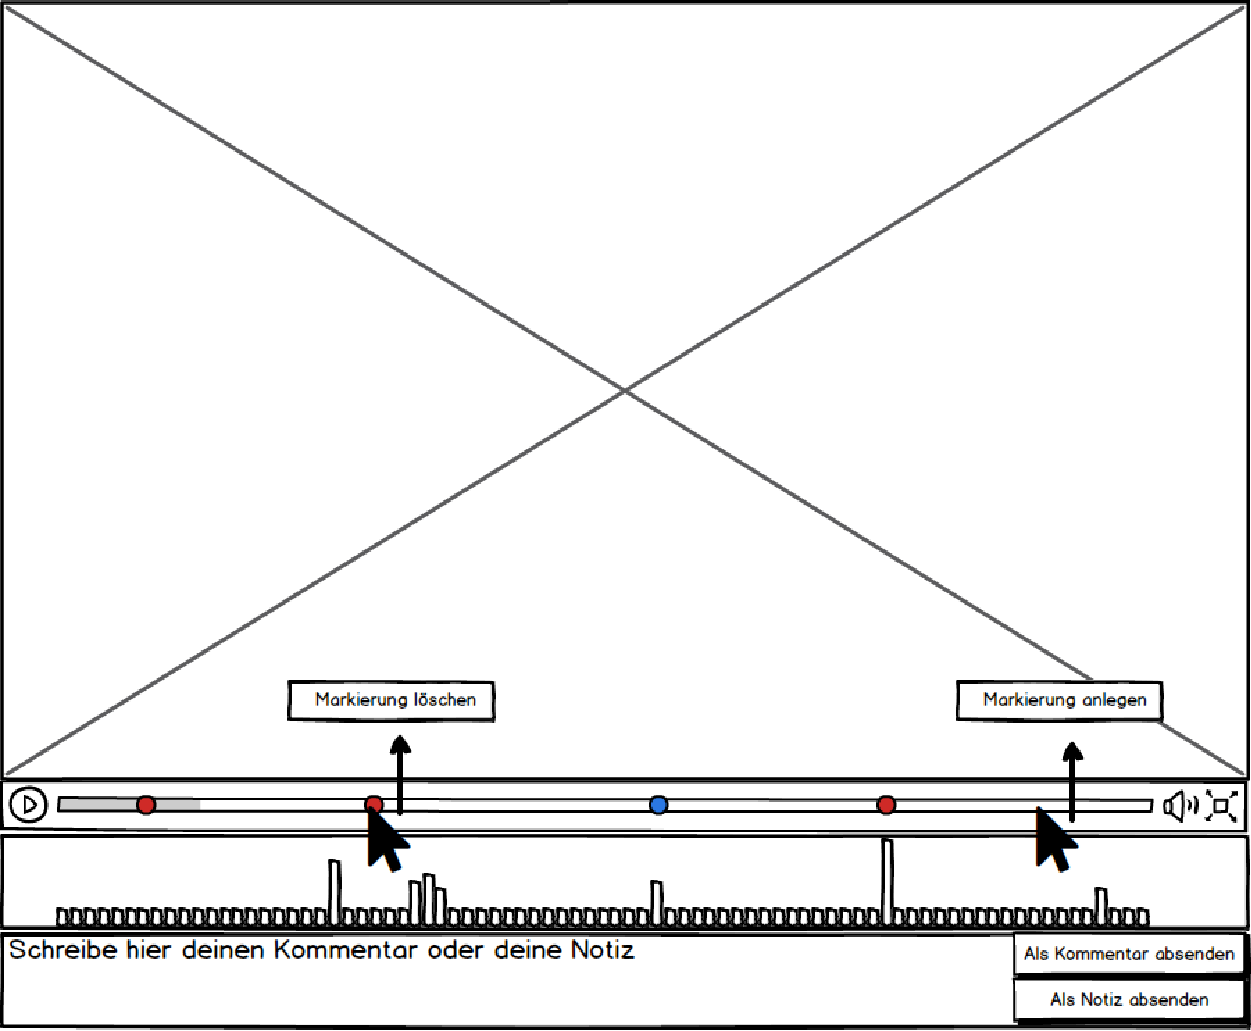
\includegraphics[width=0.8\textwidth,center]{MockupPlayerVersion1.pdf}
%\caption{\label{fig:MockupPlayerVersion1} Erster Entwurf des Players}
%\end{figure}

In einer zweiten Variante des Players wird die Visualisierung der persönlichen Notizen von der Abspielleiste in den Bereich der Kommentare verschoben. Wie in Abbildung \ref{fig:MockupPlayerVersion2} ersichtlich,  wird der Balken für den Zeitraum, in dem die persönlichen Notiz liegt, zu einem gewissen Teil blau eingefärbt. Dadurch wird nebenbei das Handling der Punkte in der Abspielleiste vereinheitlicht, da es hier nur noch die Markierungen mit Interaktionsmöglichkeit gibt.

\begin{figure}[h!]
\begin{subfigure}[c]{\textwidth}
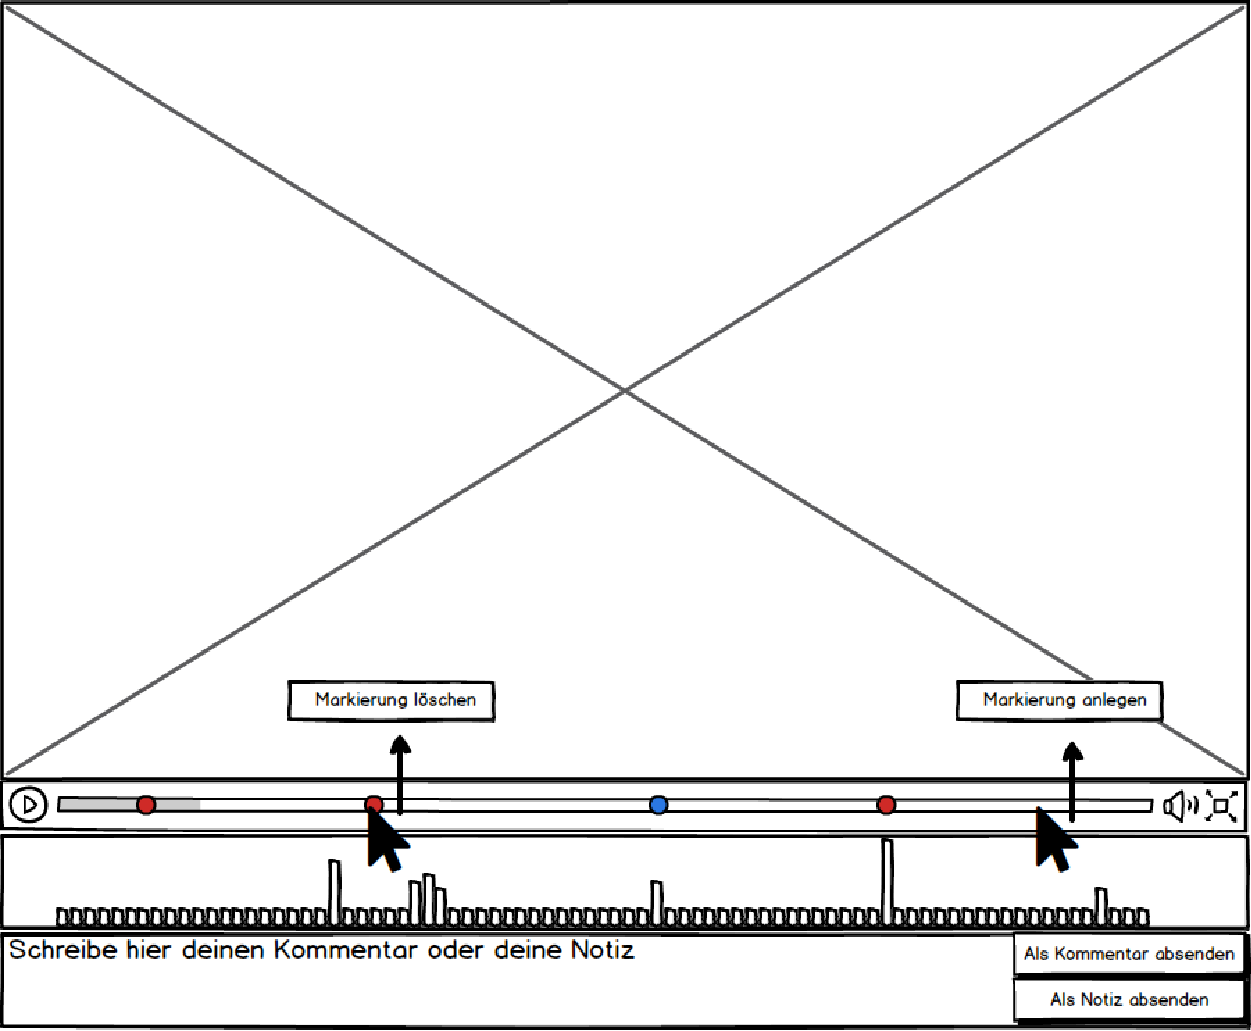
\includegraphics[width=0.8\textwidth,center]{MockupPlayerVersion1.pdf}
\subcaption{Erste Version}
\label{fig:MockupPlayerVersion1}
\end{subfigure}
\par\bigskip
\begin{subfigure}[c]{\textwidth}
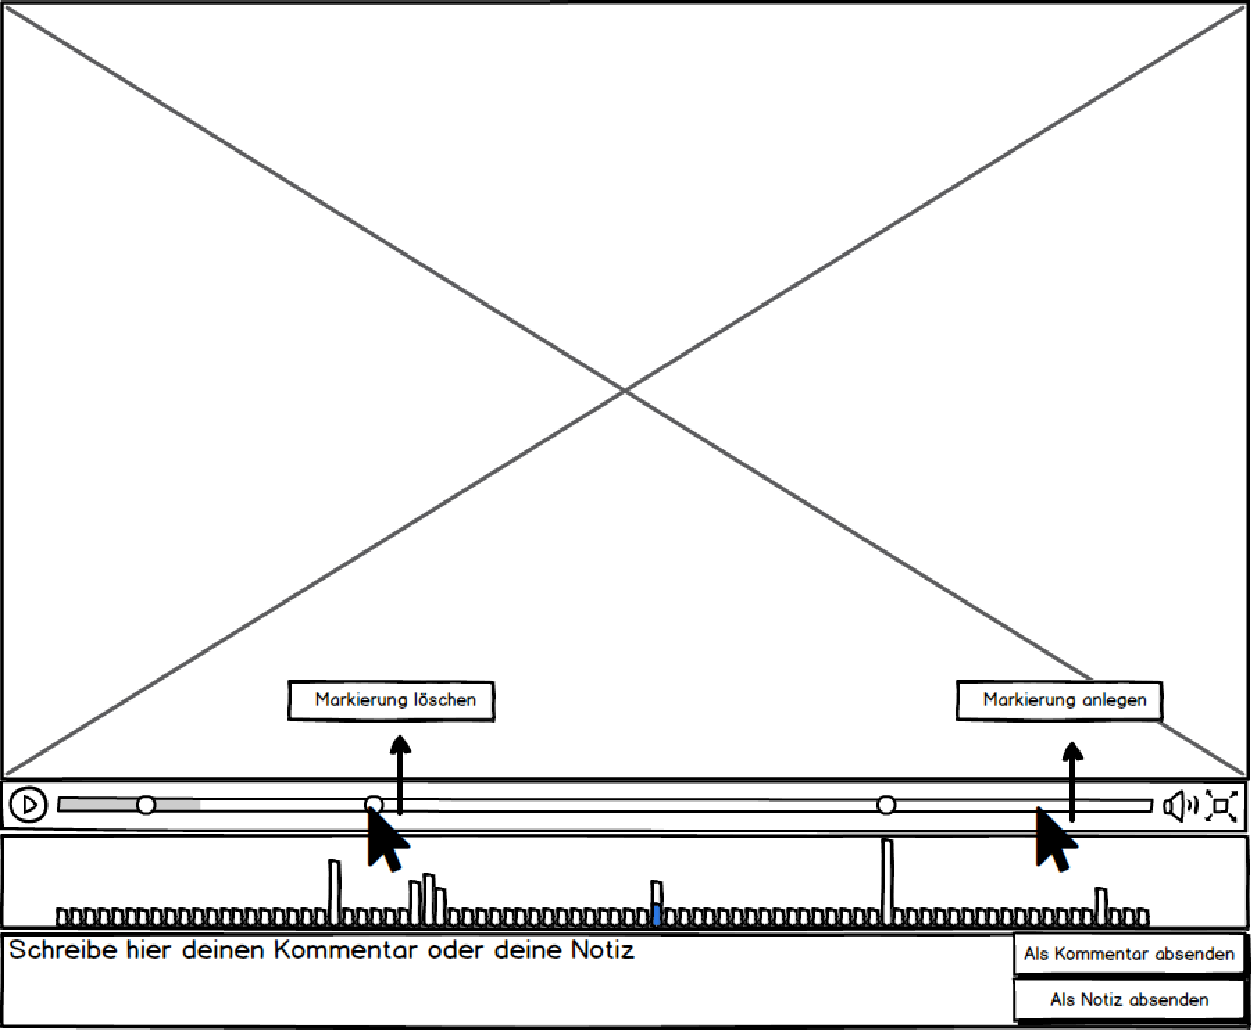
\includegraphics[width=0.8\textwidth,center]{MockupPlayerVersion2.pdf}
\subcaption{Finale Version}
\label{fig:MockupPlayerVersion2}
\end{subfigure}
\caption{Benutzeroberfläche - Player}
\label{fig:MockupPlayerVersion}
\end{figure}

%\begin{figure}[h!]
%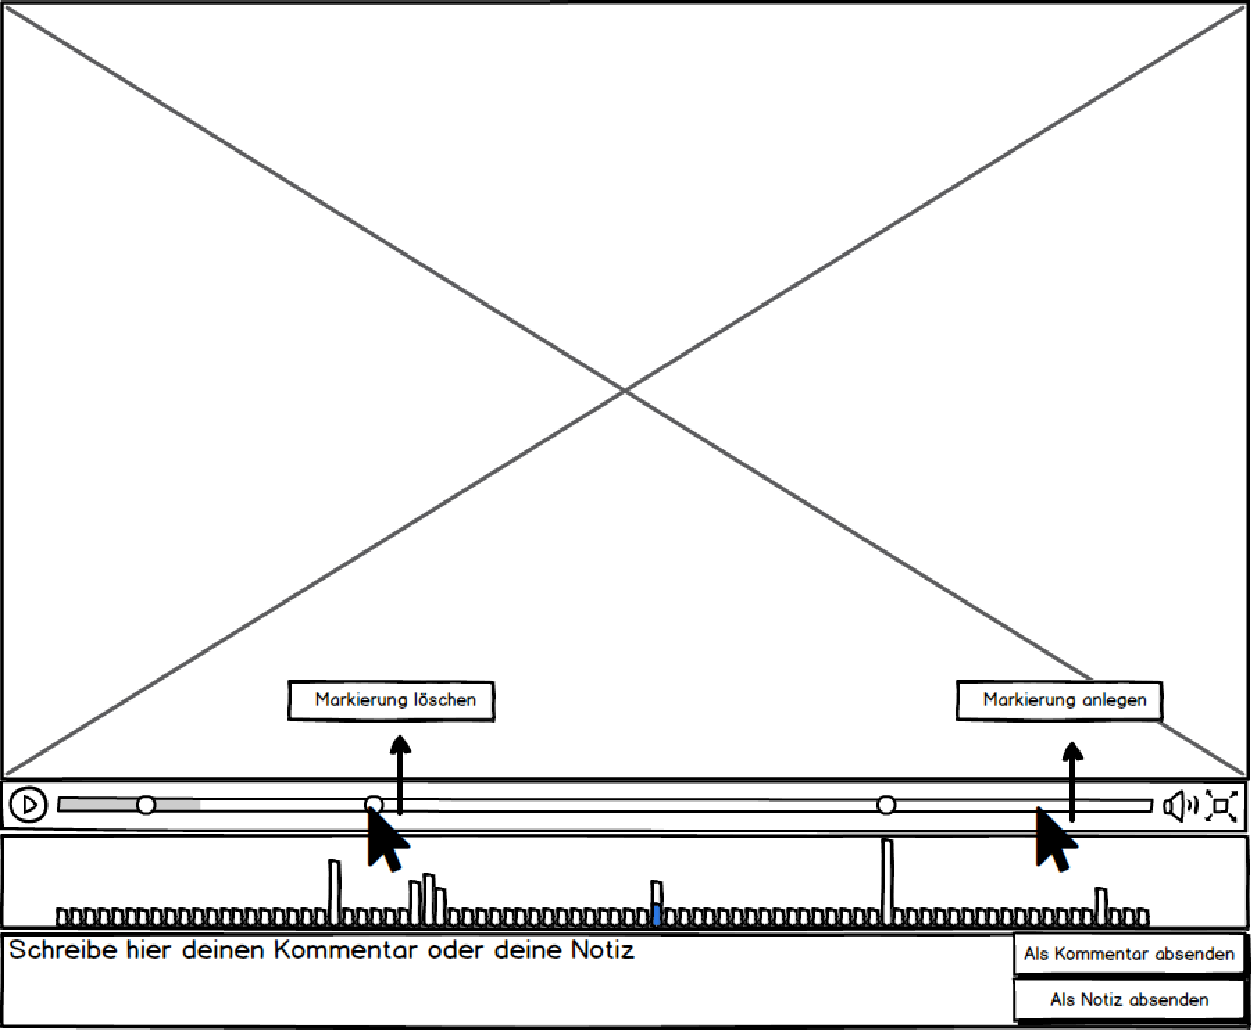
\includegraphics[width=.8\textwidth,center]{MockupPlayerVersion2.pdf}
%\caption{\label{fig:MockupPlayerVersion22}Zweiter Entwurf des Players}
%\end{figure}


%%%%%%%%%%
\subsubsection{Galerie}
Die Galerie soll dazu dienen, einen Überblick über die vorhanden Zusatzinhalte zu bieten. Die Zusatzinhalte stellen alle einen grafischen Inhalt dar. Dementsprechend kann jeder Zusatzinhalt durch ein kleines Vorschaubild repräsentiert werden. 
Eine weitere Grundfunktionalität einer Galerie ist die vergrößerte Anzeige der in der Vorschau dargestellten Inhalte, die auch in unserer Galerie zur Verfügung stehen soll. Beim Erstellen des Designs muss zusätzlich auch die Anforderung der Rückkopplung zum Player bedacht werden (siehe Abschnitt \ref{sub:AnforderungenOberflaeche}). 
%Neben der Grundfunktionalität einer Galerie, dass der ausgewählte Zusatzinhalt vergrößert angezeigt werden können soll, muss beim Erstellen des Designs auch die Anforderung der Rückkopplung zum Player bedacht werden (siehe Abschnitt \ref{sub:AnforderungenOberflaeche}). 

Die einfachste Umsetzung der Galerie ist eine Darstellung der Zusatzinhalte in einem einfachen Grid  mit Scrollbalken, wie es in Abbildung \ref{fig:MockupGalerieGrid} zu sehen ist. Zusätzlich wird das Grid um zwei Buttons für eine vergrößerte Ansicht des Zusatzinhalts sowie für die Rückkopplung zum Player ergänzt. Um eine dieser beiden Aktionen auszuführen, müsste also der gewünschte Zusatzinhalt markiert und der entsprechende Button betätigt werden.

%\begin{figure}[h!]
%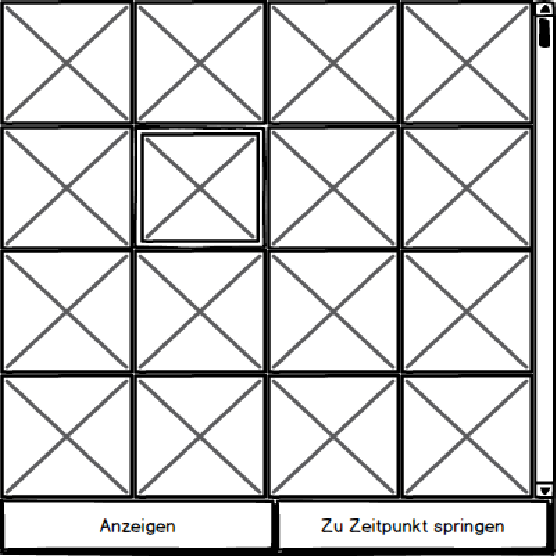
\includegraphics[width=.5\textwidth,center]{MockupGalerieGrid.pdf}
%\caption{\label{fig:MockupGalerieGrid}Garlerie als einfaches Grid}
%\end{figure}

Diese Variante hat den Vorteil, dass besonders viele Zusatzinhalte gleichzeitig angezeigt werden können. Auf der anderen Seite erhalten wir aber keinerlei Informationen zu den Zusatzinhalten. In der zweiten Variante, bei dem das Grid um einen Bereich für Details ergänzt wurde, kann man zumindest die Details des ausgewählten Zusatzinhaltes einsehen. Diese in Abbildung \ref{fig:MockupGalerieGridErweitert} erkennbaren Details sind natürlich von den vorhandenen Metadaten abhängig. Nachteil ist in diesem Fall aber, dass, durch den Bereich für die Details, bei gleicher Größe der Galerie weniger Zusatzinhalte zur selben Zeit dargestellt werden können. Das führt dazu, dass die Verwendung des Scrollbalkens häufiger notwendig wird.

%\begin{figure}[h!]
%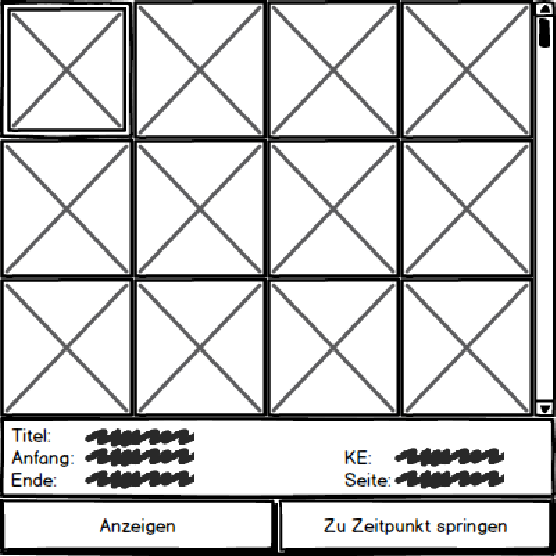
\includegraphics[width=.5\textwidth,center]{MockupGalerieGridErweitert.pdf}
%\caption{\label{fig:MockupGalerieGridErweitert}Galerie als Grid mit Bereich für Details}
%\end{figure}

Bei einer Darstellung der Zusatzinhalte als Kacheln, wie in Abbildung \ref{fig:MockupGalerieKacheln} zu sehen, können gleichzeitig für alle vorhandenen Zusatzinhalte die Details angezeigt werden. Durch diese Art der Darstellung passen jedoch noch weniger Zusatzinhalte auf die gleiche Fläche.

%\begin{figure}[h!]
%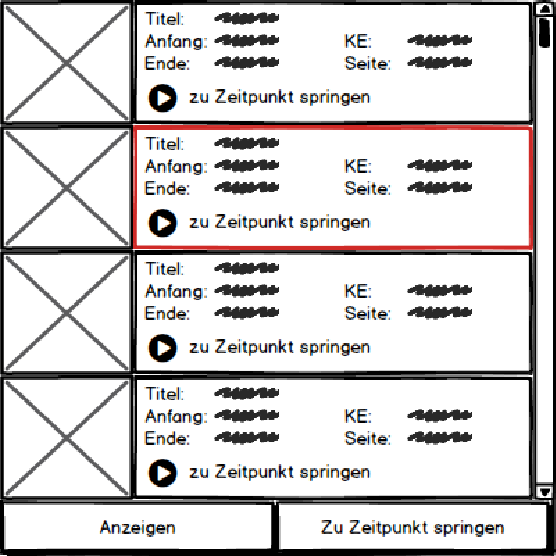
\includegraphics[width=.5\textwidth,center]{MockupGalerieKacheln.pdf}
%\caption{\label{fig:MockupGalerieKacheln}Galerie mit Darstellung in Kachelform}
%\end{figure}

Eine besonders schicke Art der Darstellung wäre die des Cover Flows, bekannt aus verschiedenen Musikplayern. In Abbildung \ref{fig:MockupGalerieCoverFlow} ist zu erkennen, dass auch hier ausschließlich Details des aktuell ausgewählten Zusatzinhaltes sichtbar sind. Des Weiteren hat diese Darstellungsweise den großen Nachteil, dass auch nicht auf einen Blick alle verfügbaren Zusatzinhalte ersichtlich sind. Dies erschwert das Durchsuchen der Zusatzinhalte ungemein. Somit ist diese Art der Darstellung zwar schön anzusehen, aber nicht sonderlich gebrauchstauglich im Zusammenhang dieser Arbeit.

%\begin{figure}[h!]
%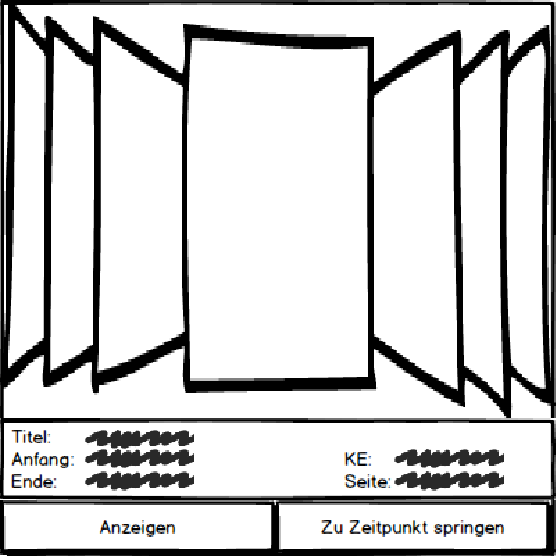
\includegraphics[width=.5\textwidth,center]{MockupGalerieCoverFlow.pdf}
%\caption{\label{fig:MockupGalerieCoverFlow}Galerie als Cover Flow}
%\end{figure}

Letztlich stellt sich die optimierte Variante der Kachel Darstellung aus Abbildung \ref{fig:MockupGalerieFinal} als beste Lösung heraus. Die Optimierung besteht daraus, dass die beiden Buttons obsolet gemacht werden. Dies kann zum einen erreicht werden, indem die vergrößerte Darstellung durch einen Klick auf die Abbildung des Zusatzinhaltes ausgelöst wird. Zum anderen bietet der Bereich der Details noch ausreichend Platz, um hier die Funktion zur Rückkopplung an den Player einzufügen. Durch diese Verbesserungen wird nicht nur mehr Platz geschaffen, sondern auch die Benutzerfreundlichkeit erhöht, indem der Vorgang zum Anzeigen der vergrößerten Ansicht beziehungsweise des Springens an den entsprechenden Zeitpunkt jeweils um einen Klick reduziert wurde.

\begin{figure}[h!]
\begin{subfigure}[c]{0.5\textwidth}
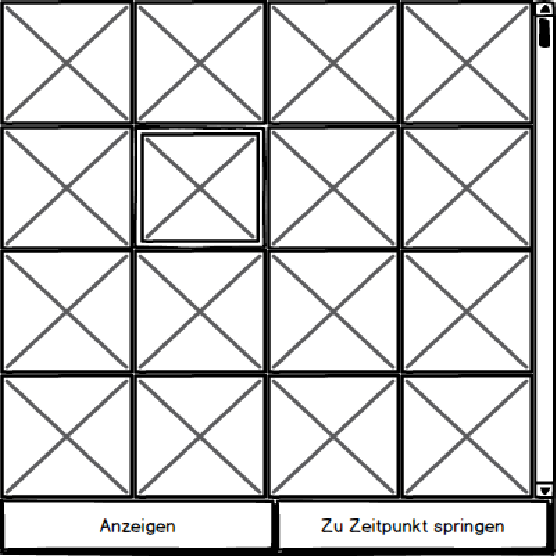
\includegraphics[width=0.8\textwidth,center]{MockupGalerieGrid.pdf}
\subcaption{Galerie als einfaches Grid}
\label{fig:MockupGalerieGrid}
\end{subfigure}%
\begin{subfigure}[c]{0.5\textwidth}
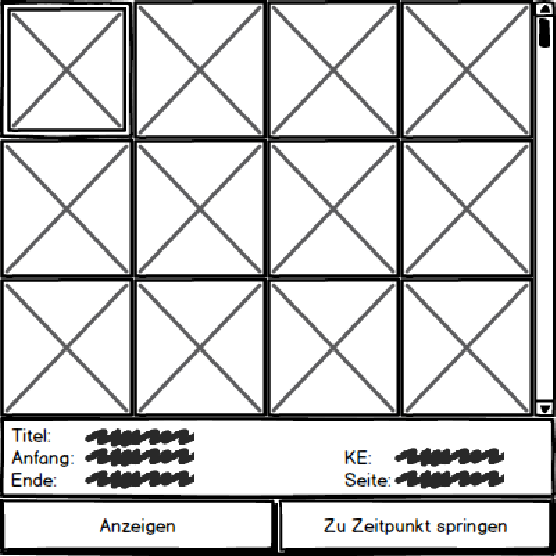
\includegraphics[width=0.8\textwidth,center]{MockupGalerieGridErweitert.pdf}
\subcaption{Galerie als Grid mit Bereich für Details}
\label{fig:MockupGalerieGridErweitert}
\end{subfigure}
\par\bigskip
\begin{subfigure}[c]{0.5\textwidth}
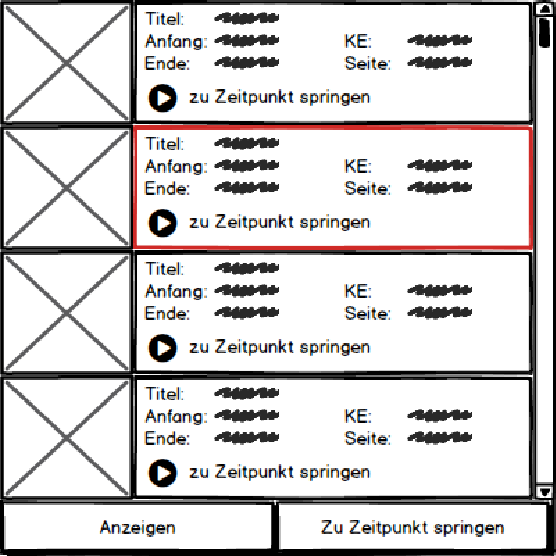
\includegraphics[width=0.8\textwidth,center]{MockupGalerieKacheln.pdf}
\subcaption{Galerie mit Darstellung in Kachelform}
\label{fig:MockupGalerieKacheln}
\end{subfigure}%
\begin{subfigure}[c]{0.5\textwidth}
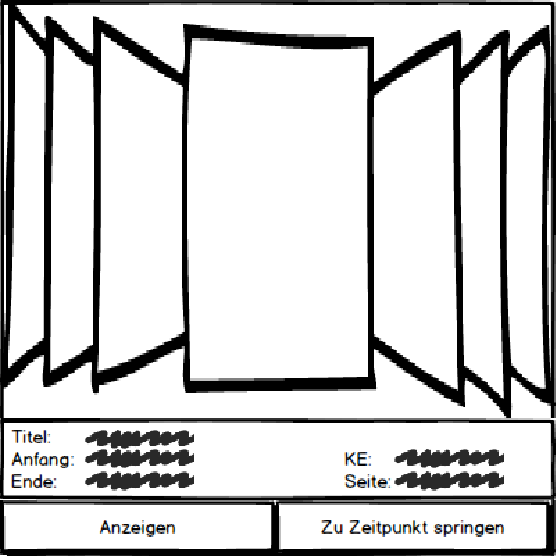
\includegraphics[width=0.8\textwidth,center]{MockupGalerieCoverFlow.pdf}
\subcaption{Galerie als Cover Flow}
\label{fig:MockupGalerieCoverFlow}
\end{subfigure}
\par\bigskip
\begin{subfigure}[c]{\textwidth}
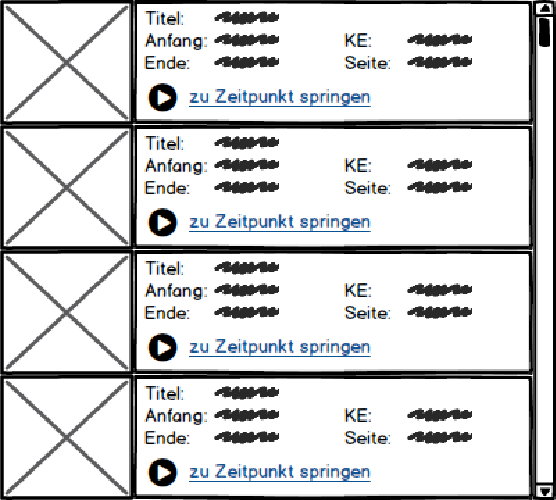
\includegraphics[width=0.4\textwidth,center]{MockupGalerieFinal.pdf}
\subcaption{Finale Version der Galerie}
\label{fig:MockupGalerieFinal}
\end{subfigure}
\caption{Benutzeroberfläche - Galerie}
\label{fig:MockupGalerie}
\end{figure}


%\begin{figure}[h!]
%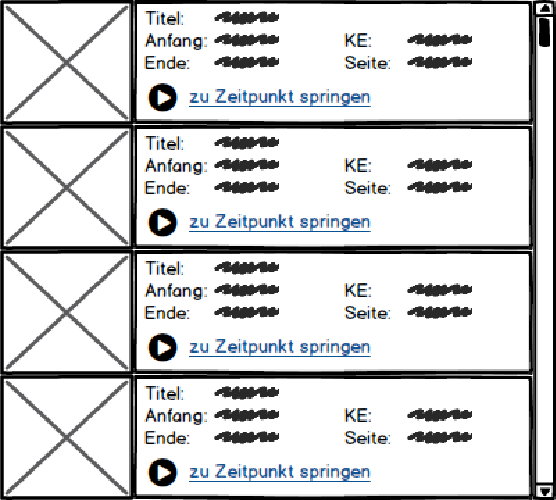
\includegraphics[width=.5\textwidth,center]{MockupGalerieFinal.pdf}
%\caption{\label{fig:MockupGalerieFinal}Finale Version der Galerie}
%\end{figure}

%%%%%%%%%%
\subsubsection{Kommentarsektion}
Die Kommentarsektion ist für die Anzeige der öffentlichen Kommentare sowie der persönlichen Notizen zuständig. Zusätzlich muss eine Suchmaske auf Basis der Anforderungen aus Abschnitt \ref{sub:AnforderungenKommentarsektion} in die Oberfläche integriert werden.

Abbildung \ref{fig:MockupKommentarsektionVersion1} zeigt eine erste Version der Kommentarsektion. Neben der Suchmaske im Kopfbereich befinden sich zwei Checkboxen. Diese ermöglichen es dem Betrachter nach öffentlichen Kommentaren und persönlichen Notizen zu filtern. Im benachbarten Dropdown-Menü kann die Grundlage der Sortierung bestimmt werden. Die Sortierung kann nach Erstellungsdatum beziehungsweise nach Zeitpunkt der Annotation innerhalb des Hyperaudio-Dokuments erfolgen. Unterhalb dieser Funktionen befindet sich die Anzeige der Kommentare und Notizen. Sowohl bei Kommentaren als auch bei Notizen wird neben dem Erstellungsdatum auch der Annotationszeitpunkt festgehalten. Dieser wird als Link umgesetzt, sodass bei einem Klick die Rückkopplung an den Player erfolgen kann. Bei Kommentaren gibt es nach Betätigung der \textit{Antworten}-Schaltfläche noch eine zusätzliche Eingabemaske zum Verfassen von Antworten. Persönliche Notizen werden durch ein Schloss-Symbol hinter dem Erstellungsdatum visualisiert. Zusätzlich befinden sich noch jeweils zwei Buttons zum Bearbeiten und Löschen auf der rechten Seite einer Notiz.

%\begin{figure}[h!]
%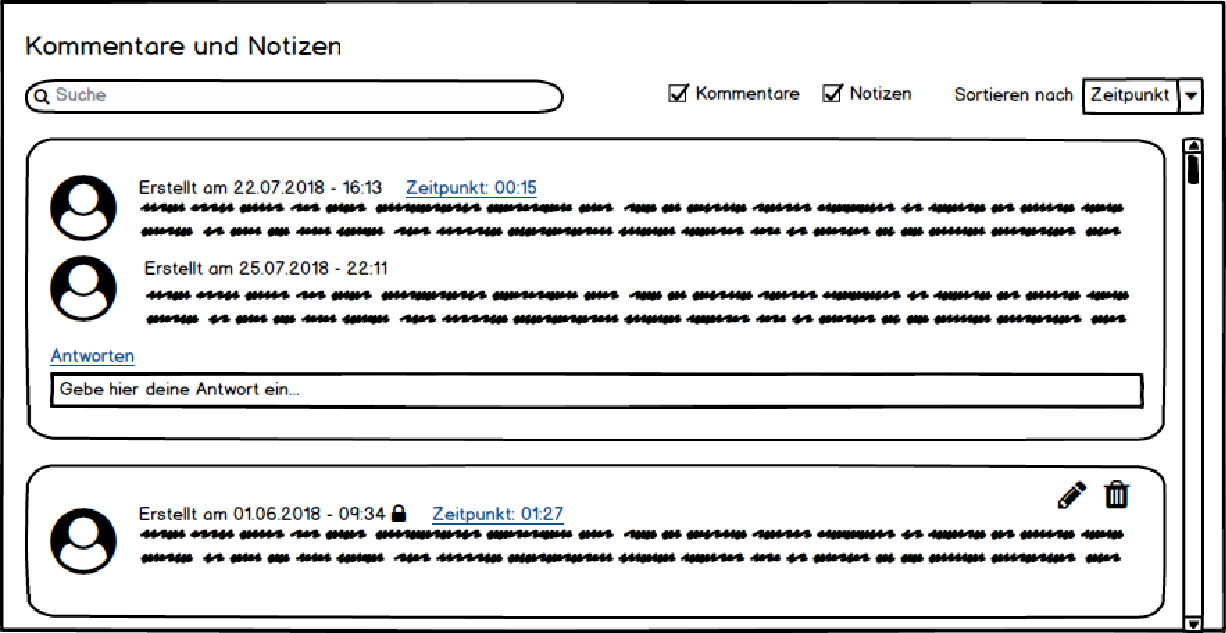
\includegraphics[width=\textwidth,center]{MockupKommentarsektionVersion1.pdf}
%\caption{\label{fig:MockupKommentarsektionVersion1}Erste Version der Kommentarsektion}
%\end{figure}

Im nochmals verbesserten Design der Kommentarsektion, welches in Abbildung \ref{fig:MockupKommentarsektionFinal} abgebildet ist, werden die Antworten auf Kommentare eingerückt dargestellt. Diese Darstellung führt zu einer besseren Übersichtlichkeit und ist auch aus anderen modernen Anwendungen bekannt.

\begin{figure}[h!]
\begin{subfigure}[c]{\textwidth}
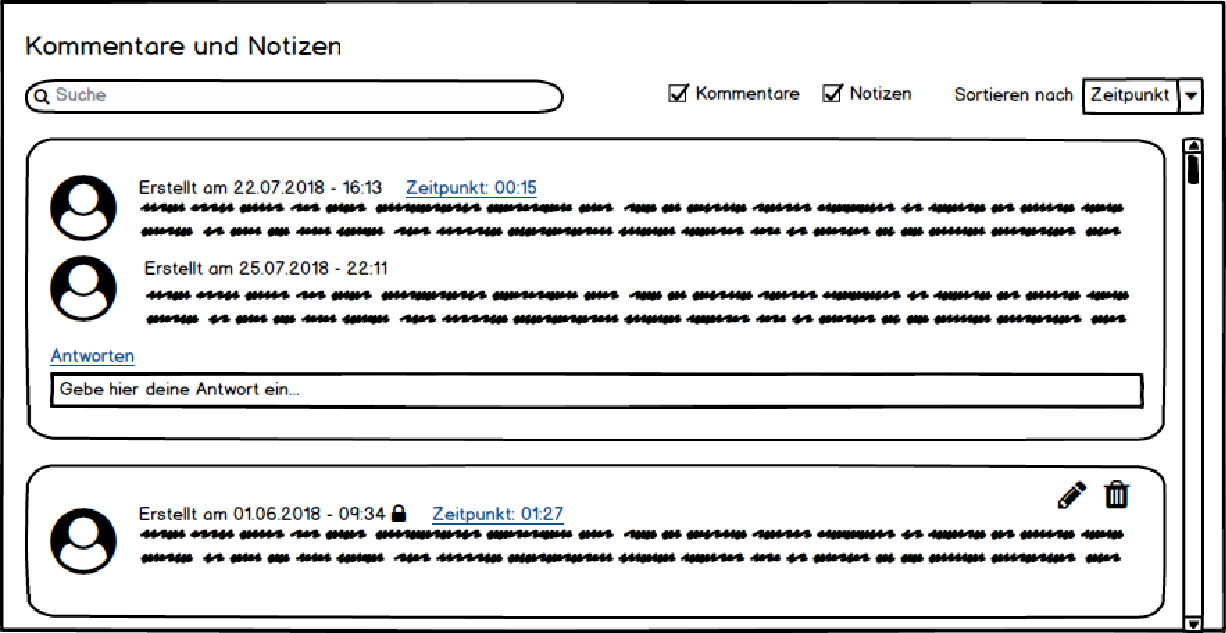
\includegraphics[width=\textwidth,center]{MockupKommentarsektionVersion1.pdf}
\subcaption{Erste Version}
\label{fig:MockupKommentarsektionVersion1}
\end{subfigure}
\par\bigskip
\begin{subfigure}[c]{\textwidth}
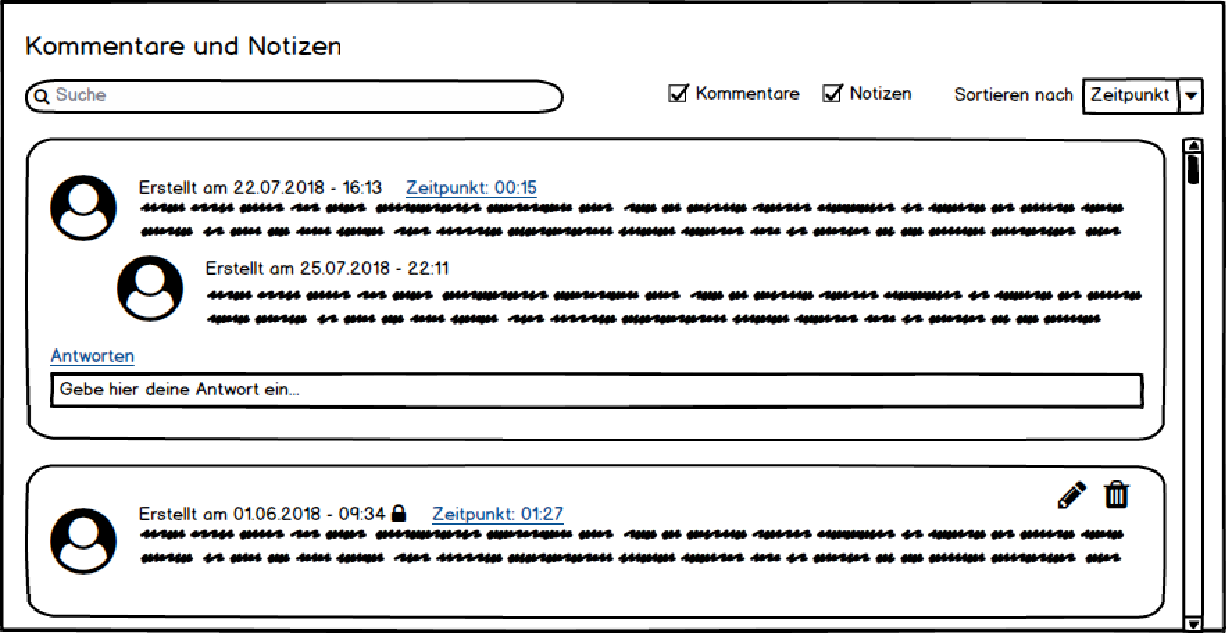
\includegraphics[width=\textwidth,center]{MockupKommentarsektionFinal.pdf}
\subcaption{Finale Version}
\label{fig:MockupKommentarsektionFinal}
\end{subfigure}
\caption{Benutzeroberfläche - Kommentarsektion}
\label{fig:MockupKommentarsektion}
\end{figure}

%\begin{figure}[h!]
%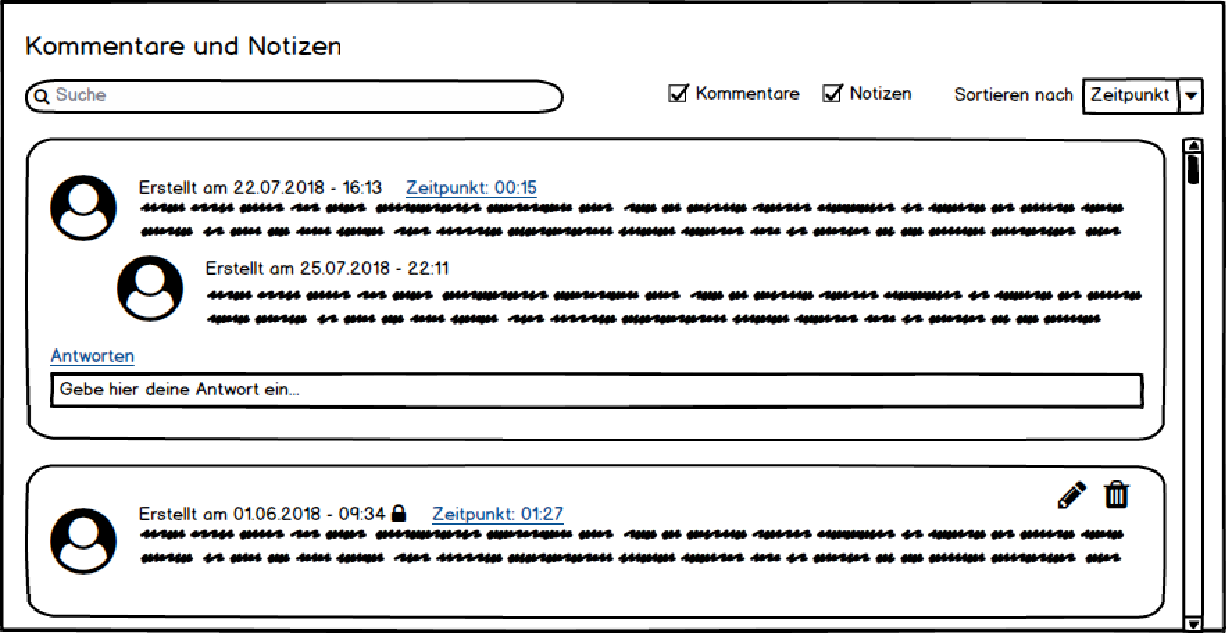
\includegraphics[width=\textwidth,center]{MockupKommentarsektionFinal.pdf}
%\caption{\label{fig:MockupKommentarsektionFinal}Finale Version der Kommentarsektion}
%\end{figure}


%%%%%%%%%%
\subsubsection{Zusammenführen der Elemente}
Im ersten Schritt führen wir die jeweils favorisierten Elemente in ein Layout zusammen. Dabei orientieren wir uns zunächst an unserer grobe Skizze aus Kapitel \ref{cha:analyse}. Wie nun in Abbildung \ref{fig:MockupSeiteLayoutVersion1} zu erkennen ist, ist die Kommentarsektion so in die Breite gezogen, dass das Lesen der Inhalte unangenehm werden kann. Aus diesem Grund wird in der finalen Version (siehe Abbildung \ref{fig:MockupSeiteLayoutFinal}) die Breite der Kommentarsektion auf die Breite des Players beschränkt. Dies hat zeitgleich zur Folge, dass der nun vorhandene freie Platz für die Galerie verwendet werden kann. Spätestens hiermit wird der Nachteil der gewählten Darstellungsweise der Galerie egalisiert, da nun ausreichend viele Zusatzinhalte ohne die Verwendung des Scrollbalkens eingesehen werden können.

%\begin{figure}[h!]
%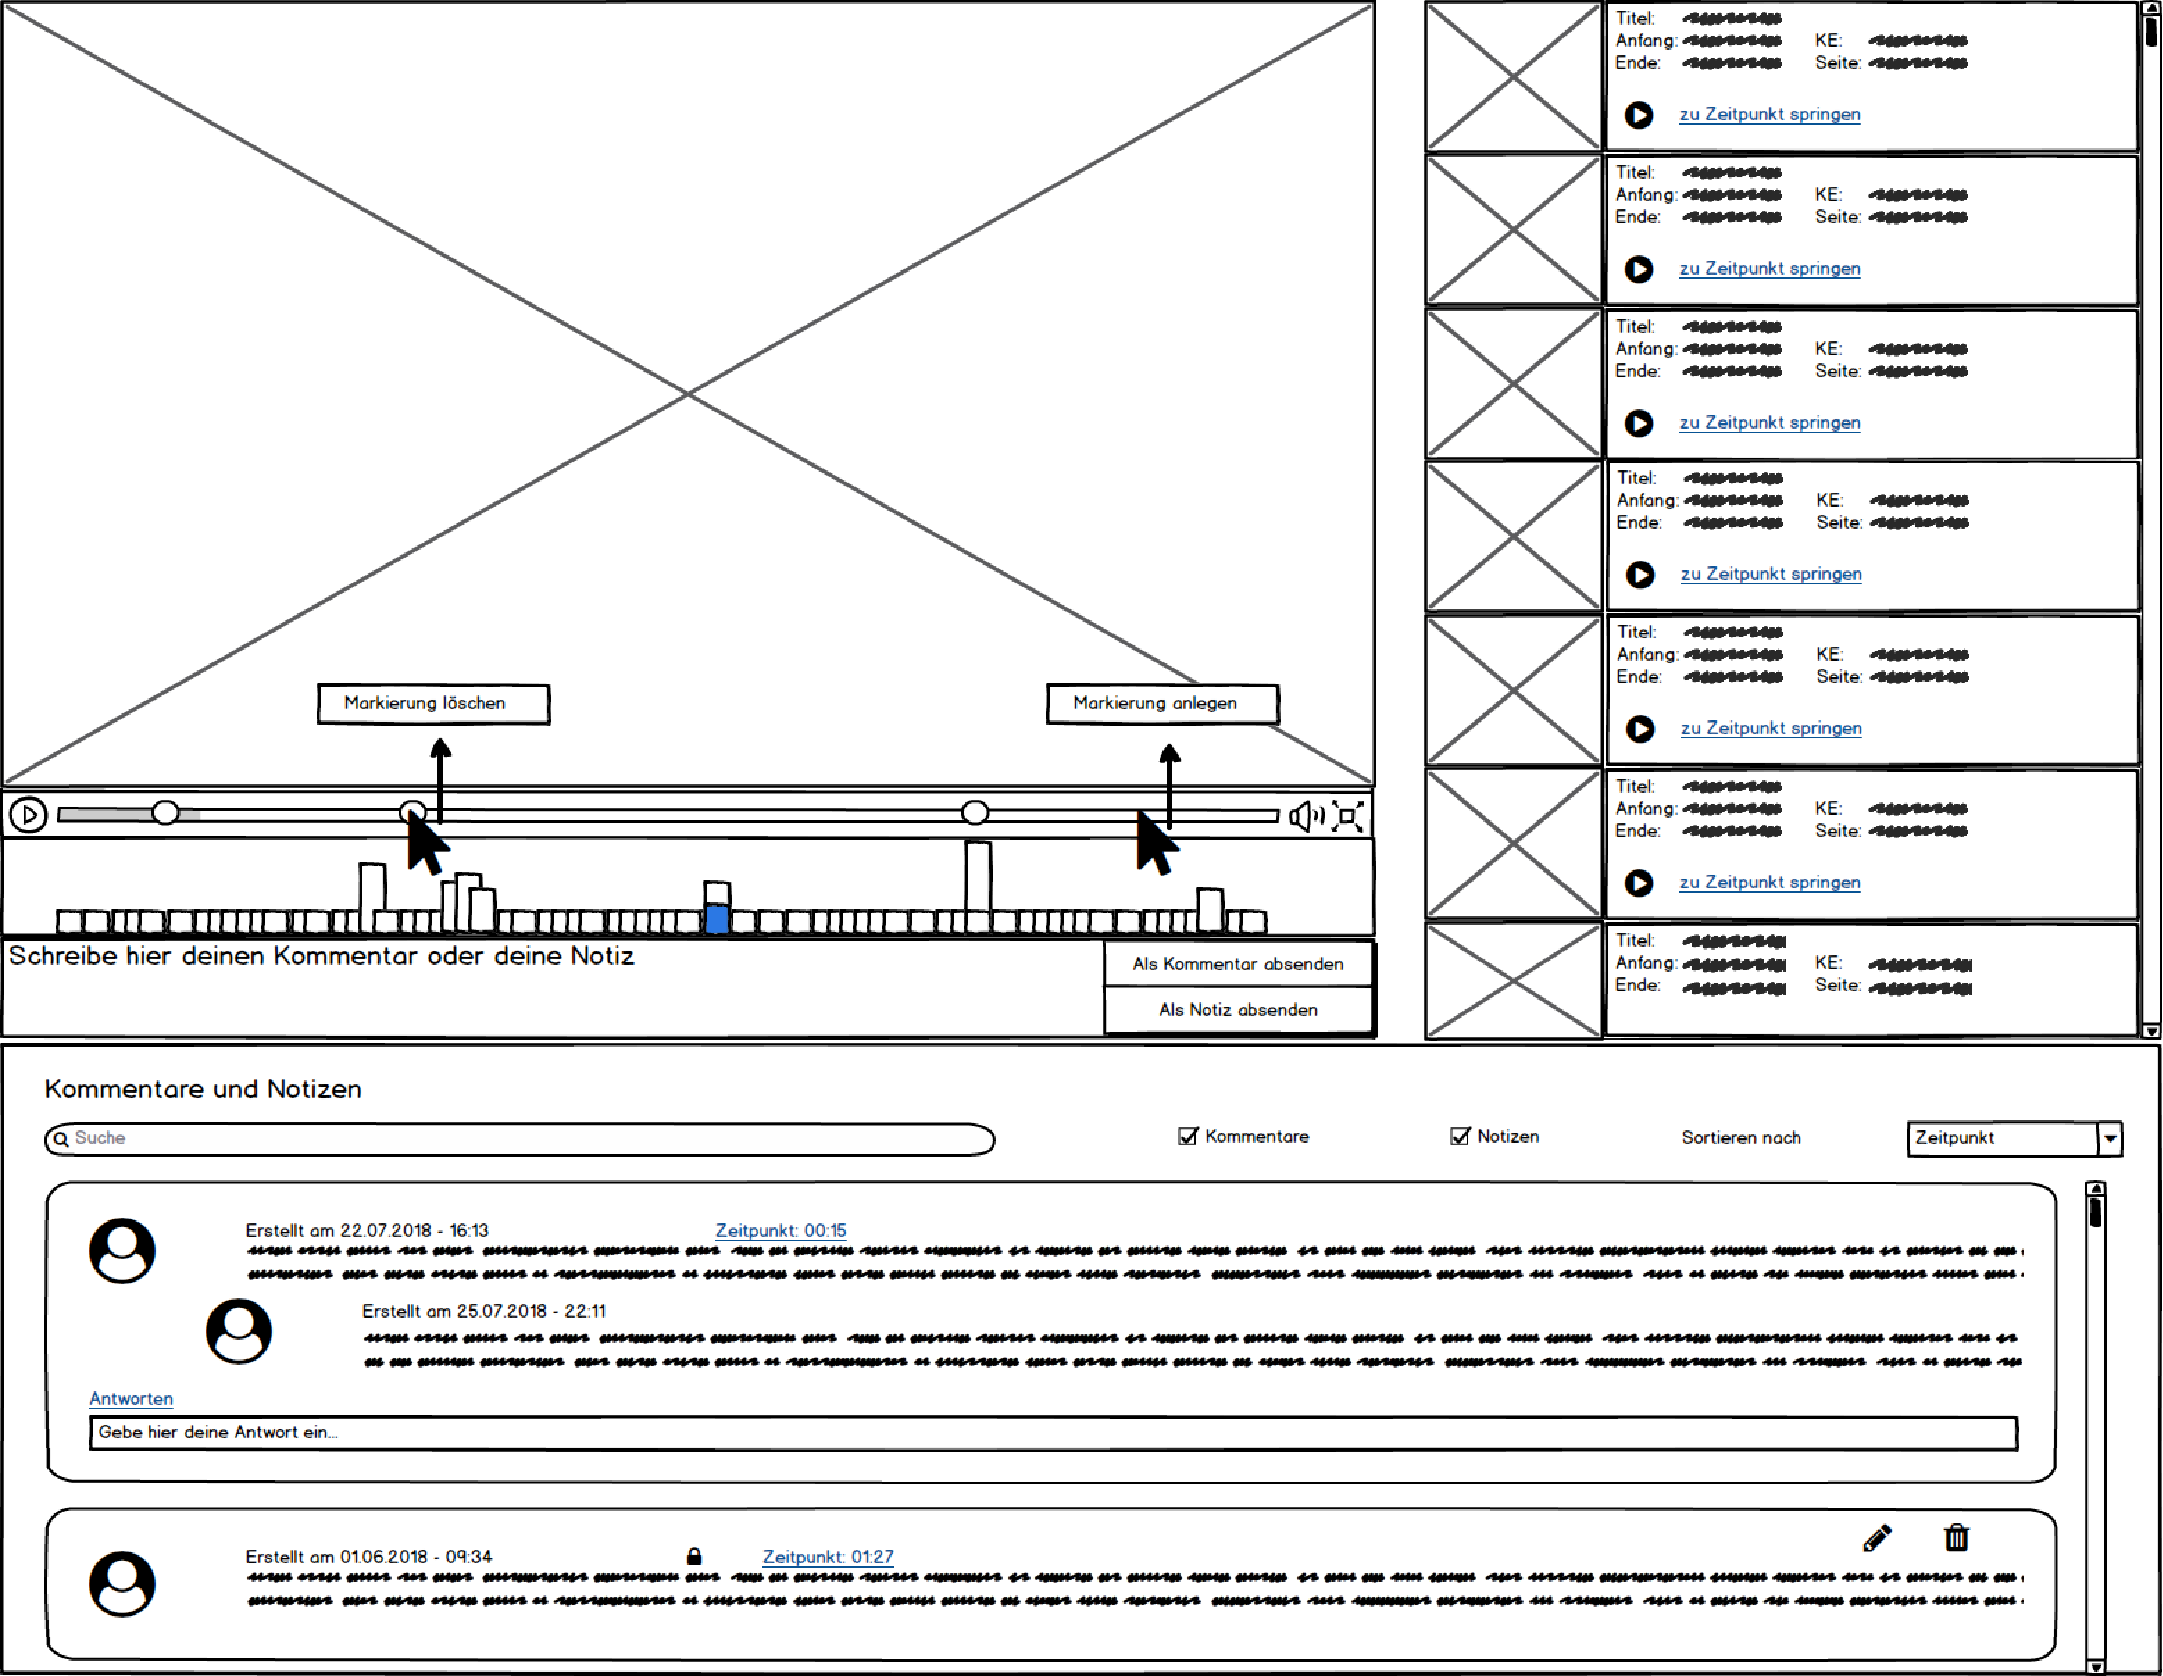
\includegraphics[width=\textwidth,center]{MockupSeiteLayoutVersion1.pdf}
%\caption{\label{fig:MockupSeiteLayoutVersion1}Erstes Layout der Seite für Hyperaudio-Dokumente}
%\end{figure}

%\begin{figure}[h!]
%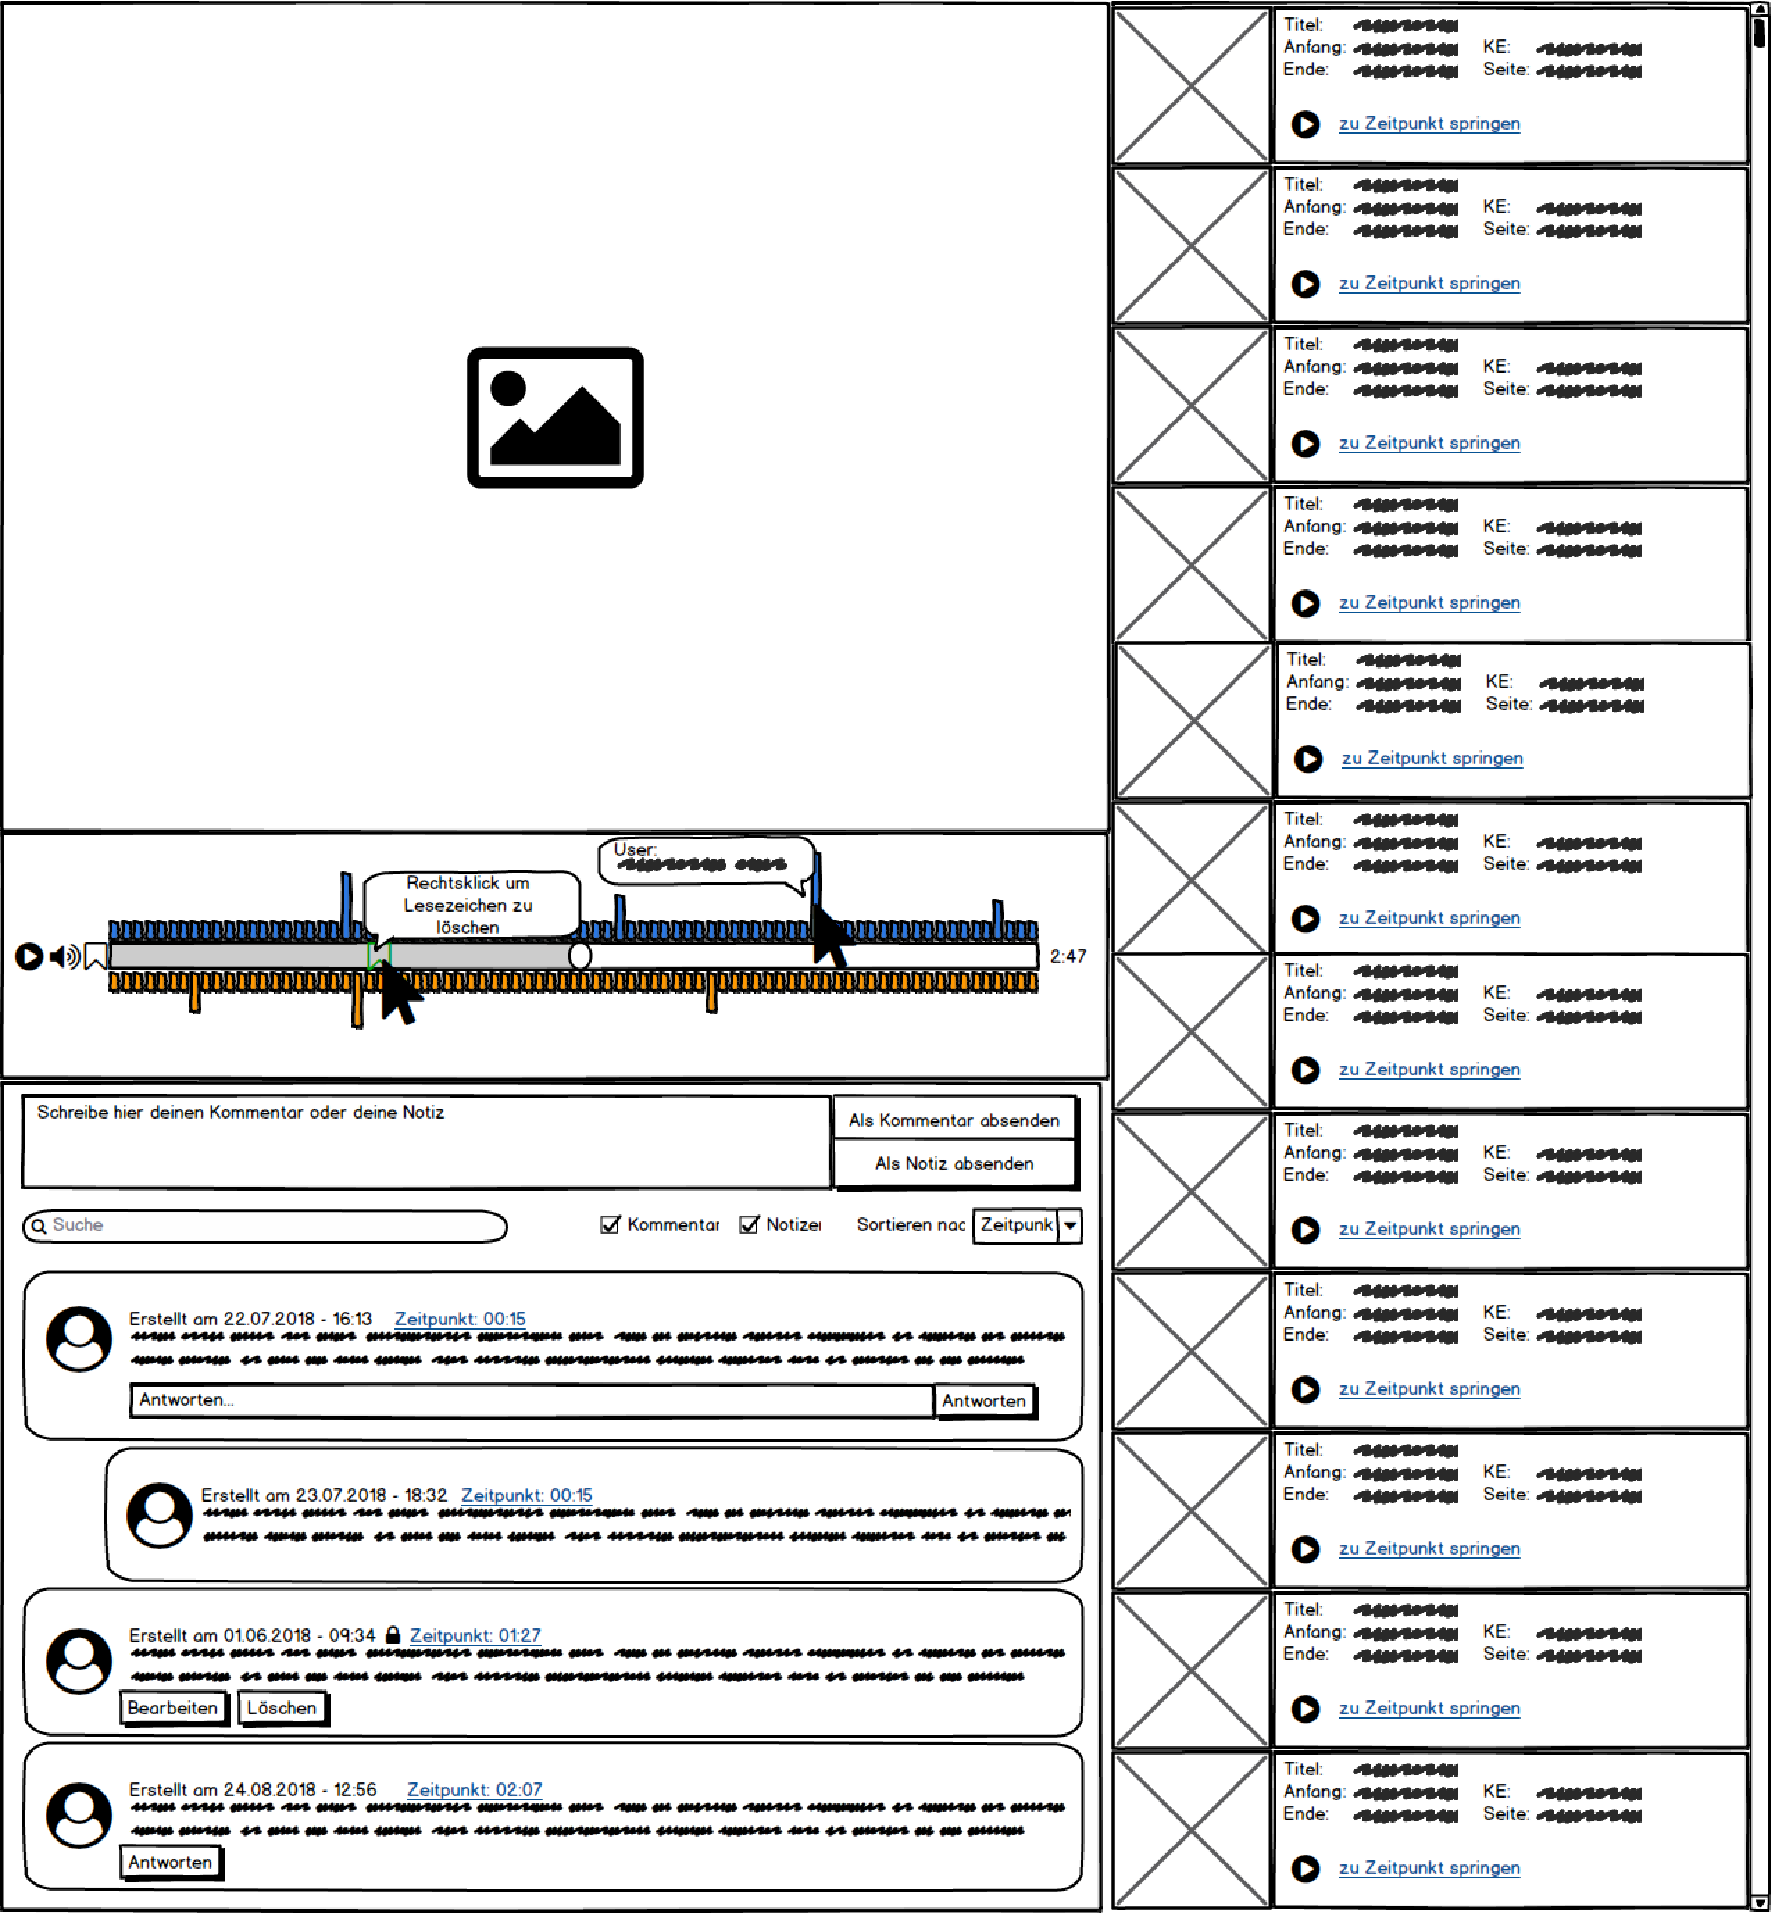
\includegraphics[width=\textwidth,center]{MockupSeiteLayoutFinal.pdf}
%\caption{\label{fig:MockupSeiteLayoutFinal}Finales Layout der Seite für Hyperaudio-Dokumente}
%\end{figure}

\begin{figure}[h!]
\begin{subfigure}[c]{\textwidth}
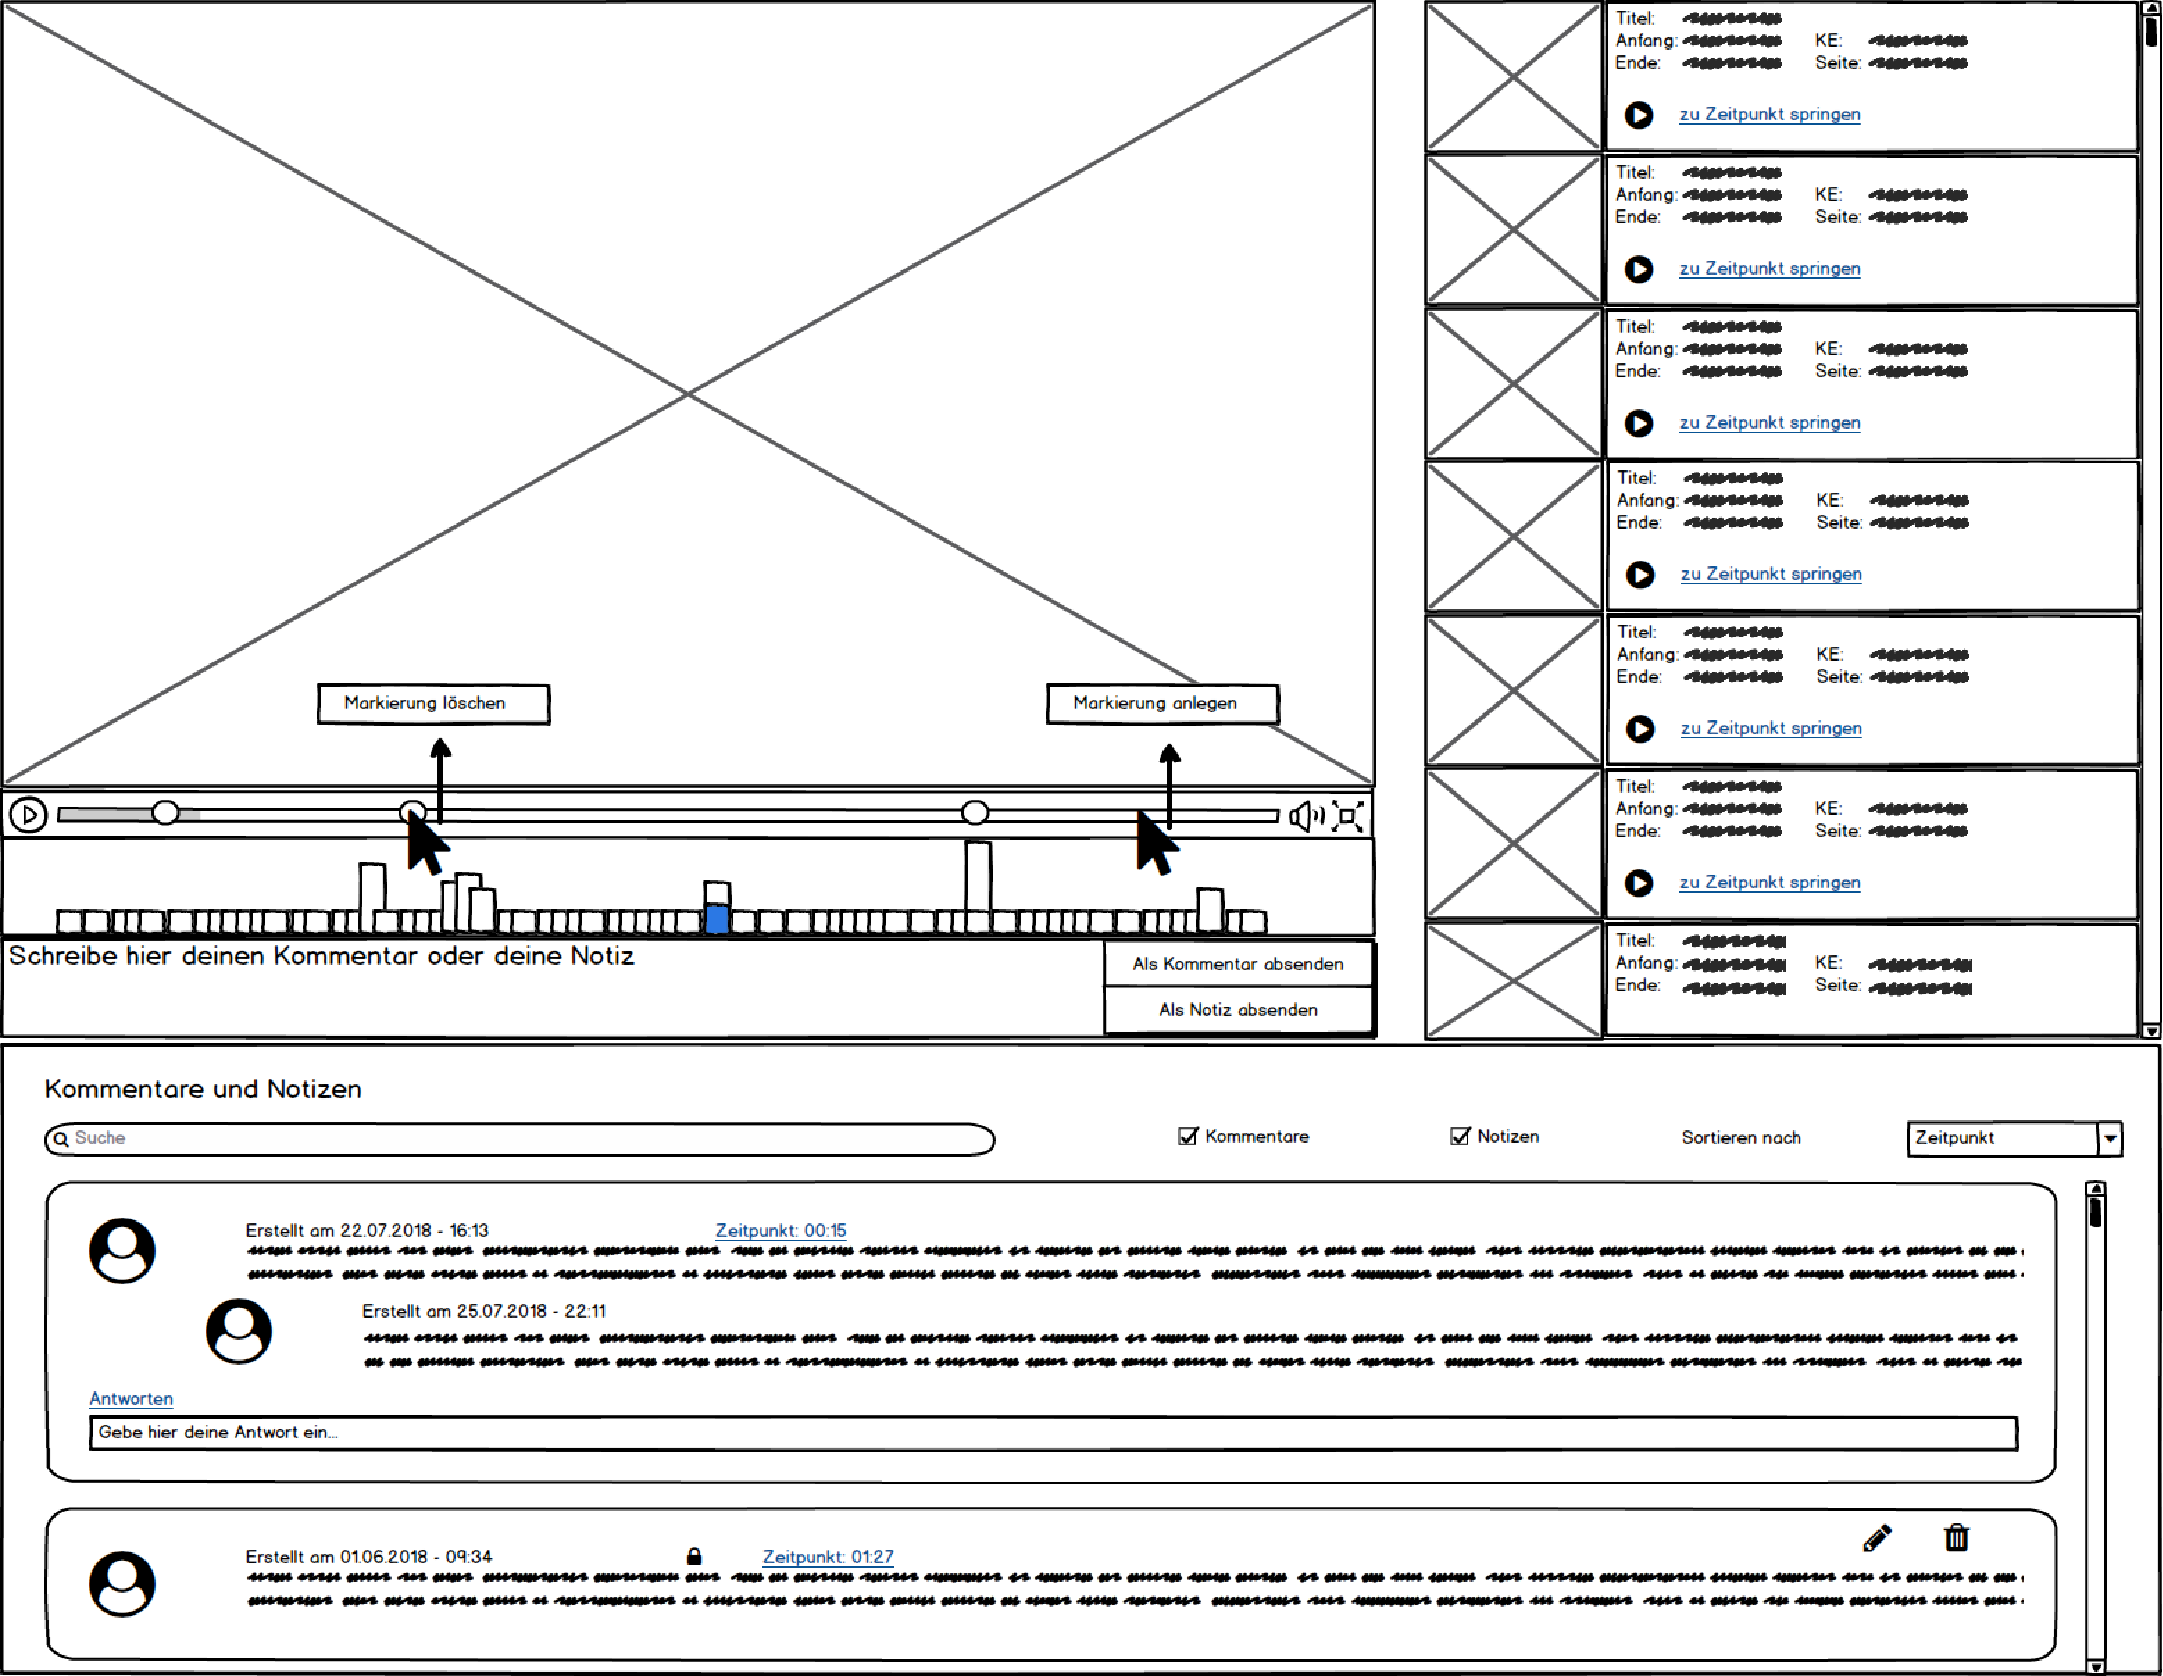
\includegraphics[width=0.9\textwidth,center]{MockupSeiteLayoutVersion1.pdf}
\subcaption{Erste Version}
\label{fig:MockupSeiteLayoutVersion1}
\end{subfigure}
\par\bigskip
\begin{subfigure}[c]{\textwidth}
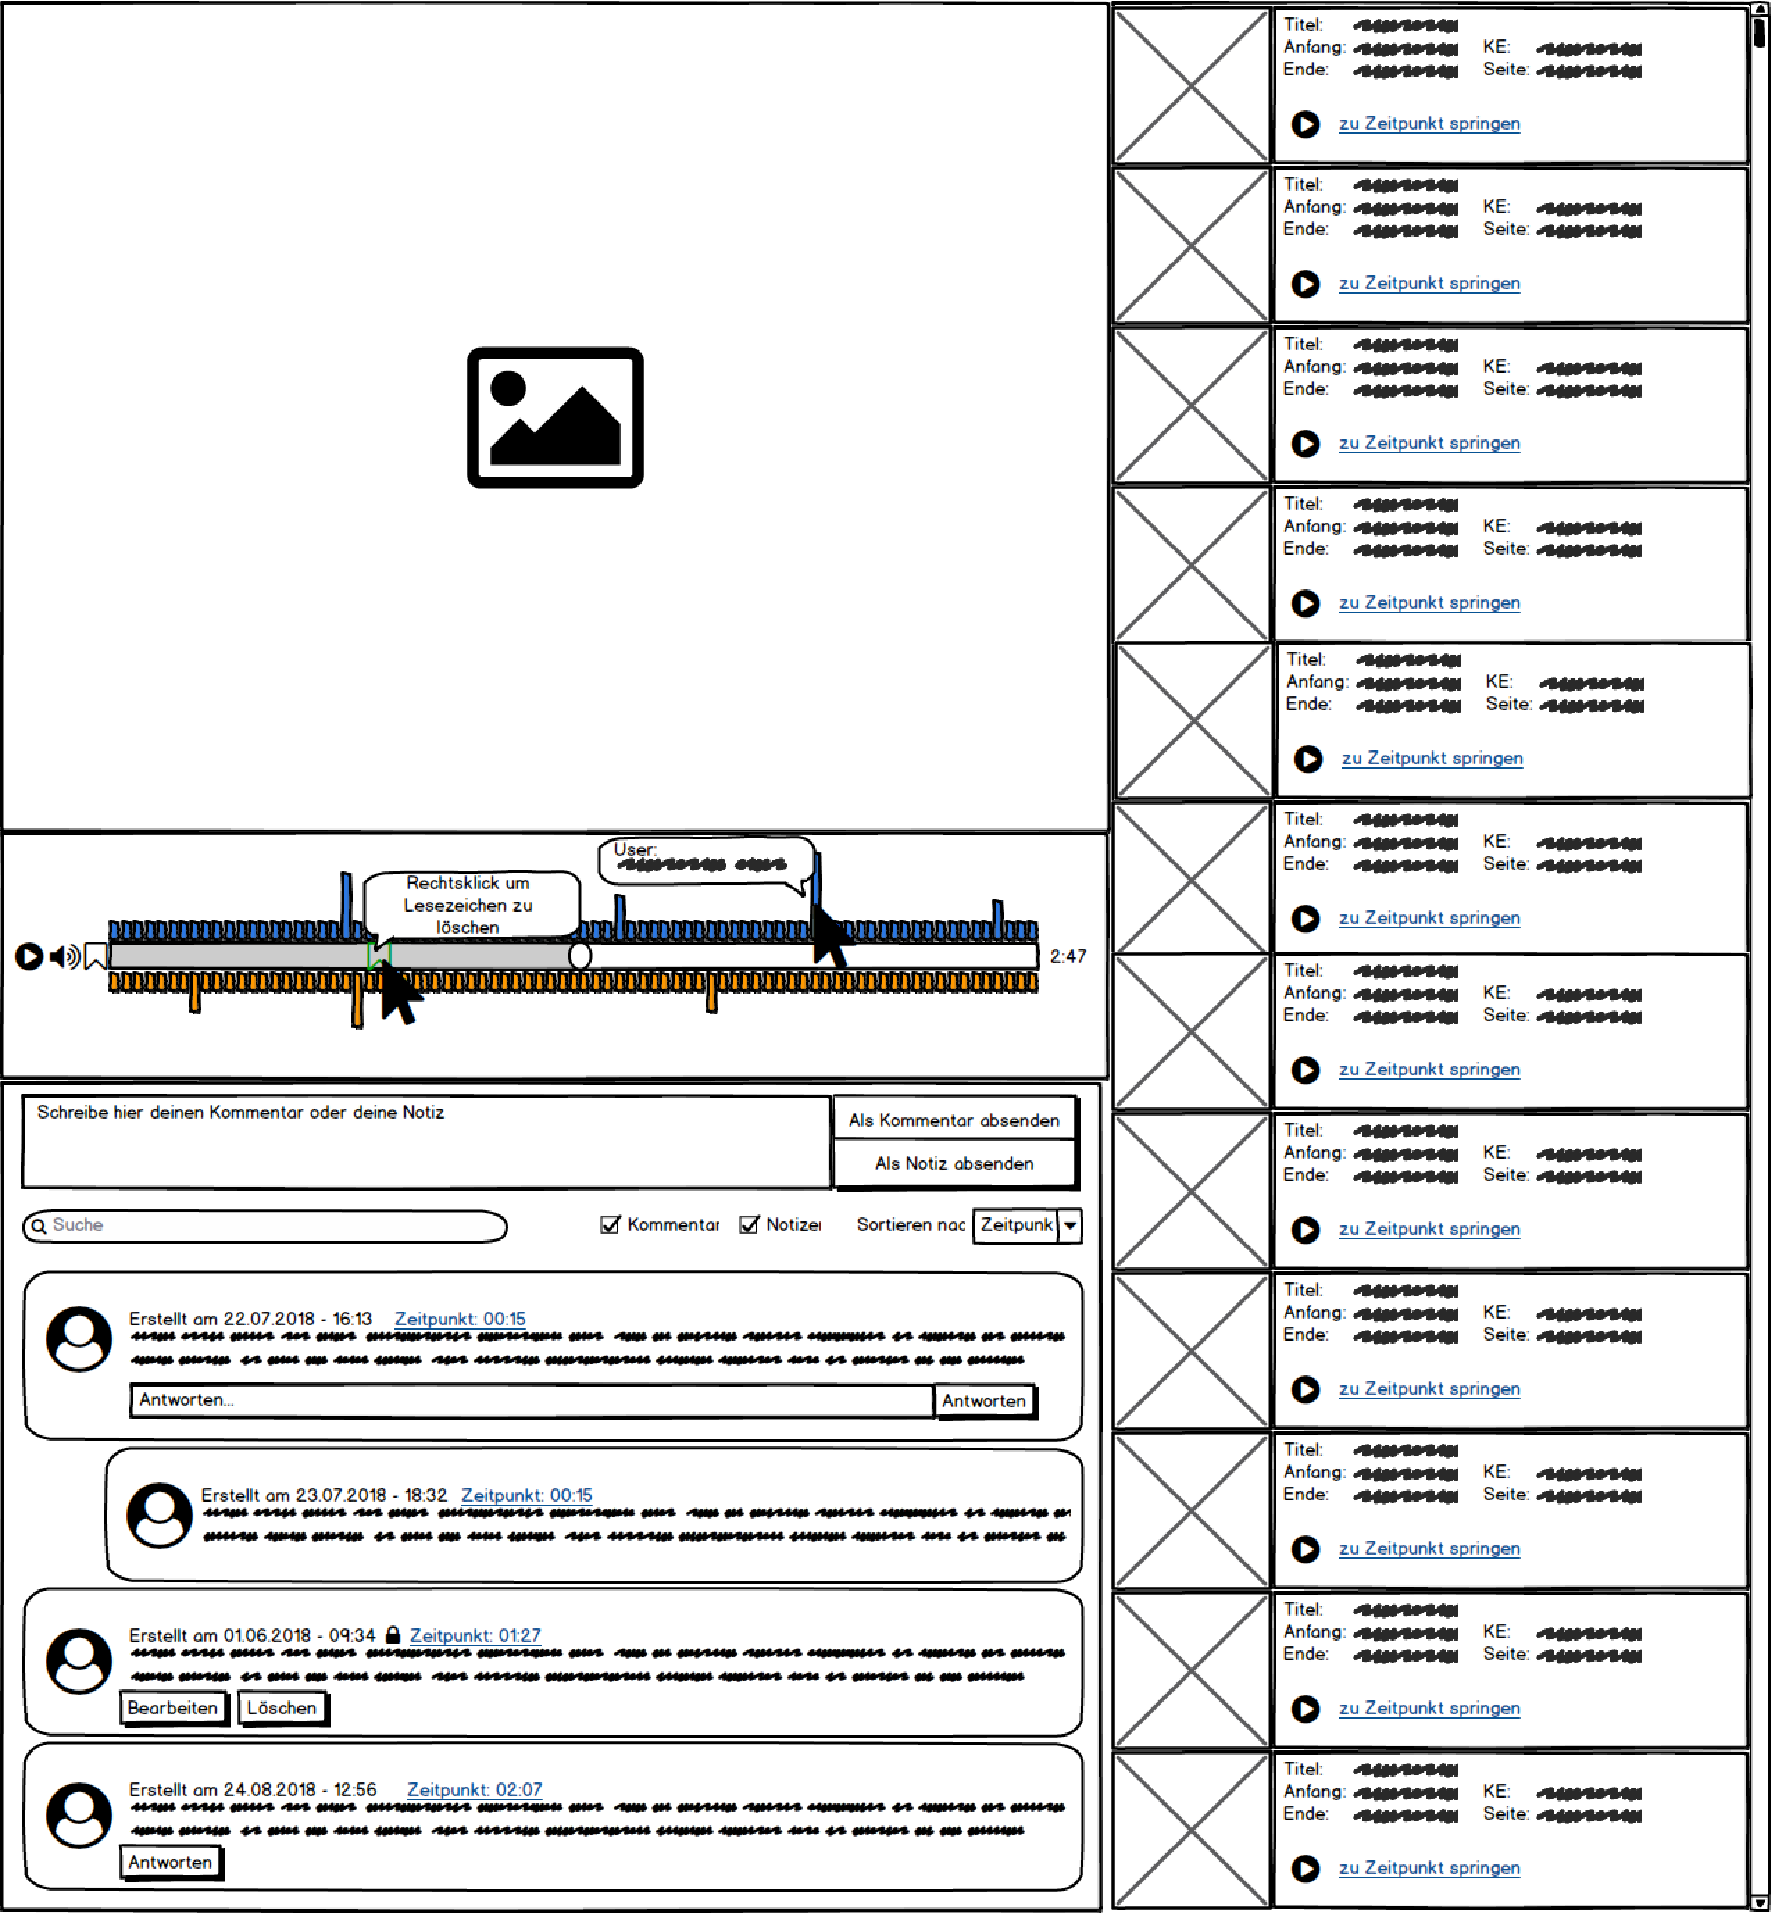
\includegraphics[width=0.9\textwidth,center]{MockupSeiteLayoutFinal.pdf}
\subcaption{Finale Version}
\label{fig:MockupSeiteLayoutFinal}
\end{subfigure}
\caption{Benutzeroberfläche - Layout der Seite für Hyperaudio-Dokumente}
\label{fig:MockupSeiteLayout}
\end{figure}

%%%%%%%%%%
\subsection{Administrationsseite eines Hyperaudio-Dokuments}
\dots


%%%%%%%%%%
\subsection{Moodle-Oberfläche im Allgemeinen}
\dots


%%%%%%%%%%
\section{Architektur des Moodle-Plugins}
\dots


%%%%%%%%%%
\section{Definition des Schnittstellenformats für Hyperaudio-Dokumente}
\dots




%%%%%%%%%%%%%%%%
\chapter{Implementierung}
%% lade Kapitel aus Datei
%%%%%%%%%%
\section{Moodle-Integration}
\dots


%%%%%%%%%%
\section{Player}
\dots


%%%%%%%%%%
\section{Kommentarsektion}
\dots


%%%%%%%%%%
\section{Evaluation}
\dots


%%%%%%%%%%%%%%%%
\chapter{Zusammenfassung und Ausblick}
%% lade Kapitel aus Datei
\dots



%%%%%%%%%%%%%%%% ANHANG
\appendix

%%
\chapter{Erster Teil des Anhangs}
\dots

%%
\chapter{Zweiter Teil des Anhangs}
\dots




%%% Verzeichnisse
\backmatter
\pagestyle{fancyclear}



%% Literaturverzeichnis
%\phantomsection\addcontentsline{toc}{chapter}{Literaturverzeichnis}
{\footnotesize\flushleft\setlength{\itemsep}{-3pt}%\setlength{\bibsep}{3pt}
\bibliographystyle{plainnat}
\bibliography{literatur}}
\cleardoublepage


%% Abbildungsverzeichnis
\phantomsection\addcontentsline{toc}{chapter}{Abbildungsverzeichnis}
\listoffigures
\cleardoublepage


%% Tabellenverzeichnis
\phantomsection\addcontentsline{toc}{chapter}{Tabellenverzeichnis}
\listoftables
\cleardoublepage


%% Auflistungsverzeichnis
\phantomsection\addcontentsline{toc}{chapter}{Auflistungsverzeichnis}
\renewcommand\lstlistlistingname{Verzeichnis der Auflistungen}
\lstlistoflistings
\cleardoublepage


%% Verzeichnis von Algorithmen
\phantomsection\addcontentsline{toc}{chapter}{Verzeichnis der Algorithmen}
\renewcommand*\listalgorithmcfname{Verzeichnis der Algorithmen}
\listofalgorithms
\cleardoublepage


%% Abkürzungsverzeichnis
\phantomsection\addcontentsline{toc}{chapter}{Abkürzungsverzeichnis}
\chapter*{Abkürzungsverzeichnis}

%\begin{description}
%%\item[AICC] Aviation Industry Computer-Based Training Committee
%%\item[AJAX] Asynchronous JavaScript and XML
%%\item[API] Application Programing Interface
%%\item[BMBF] Bundesministerium für Bildung und Forschung
%\end{description}
\cleardoublepage


%% Erklärung ...
Name: \thesisauthor \hfill Matrikelnummer: \thesismatrikelnummer \vspace{2cm}
\subsection*{Eidesstattliche Erklärung}
Ich erkläre hiermit, dass ich diese \thesistype~selbständig verfasst, noch nicht anderweitig für Prüfungszwecke vorgelegt, keine anderen als die angegebenen Quellen und Hilfsmittel benutzt sowie wörtliche und sinngemäße Zitate als solche gekennzeichnet habe.\\[1cm]
Hagen, den \dotfill

\hspace{2cm}{\footnotesize Datum}\hspace{5cm} {\footnotesize \thesisauthor}



\end{document}
